% !TeX encoding = UTF-8
% !TeX program = xelatex
% !TeX spellcheck = en_US

\documentclass[degree=master,degree-type=professional,fontset=ubuntu]{ustcthesis}
% degree      = doctor | master | bachelor
% degree-type = academic | professional
% language    = chinese | english
% fontset     = windows | mac | ubuntu | fandol

% 加载宏包、全部的配置
% !TeX root = ./main.tex

\ustcsetup{
  title              = {基于乐观锁的内存数据库\\索引模块设计与实现},
  title*             = {Design and Implementation of In-Memory Database Index Module Based on Optimistic Lock},
  author             = {XXX},
  author*            = {XXX},
  speciality         = {软件工程},
  speciality*        = {Software Engineering},
  supervisor         = {XXX~XXX},
  supervisor*        = {XXX},
  % date               = {2017-05-01},  % 默认为今日
  % professional-type  = {专业学位类型},
  % professional-type* = {Professional degree type},
  % department         = {软件学院},  % 院系,本科生需要填写
  % student-id         = {XXX},  % 学号,本科生需要填写
  % secret-level       = {秘密},     % 绝密|机密|秘密|控阅,注释本行则公开
  % secret-level*      = {Secret},  % Top secret | Highly secret | Secret
  % secret-year        = {10},      % 保密/控阅期限
  %
  % 数学字体
  % math-style         = GB,  % 可选:GB, TeX, ISO
  math-font          = xits,  % 可选:stix, xits, libertinus
}


% 加载宏包

% 定理类环境宏包
\usepackage{amsthm}

% 插图
\usepackage{graphicx}

% 绘图
\usepackage{pgfplots}
\usepackage{tikz}
\pgfplotsset{width=6.6cm,compat=1.7}

% 三线表
\usepackage{booktabs}

% 跨页表格
\usepackage{longtable}

% 算法
% \usepackage[ruled,linesnumbered]{algorithm2e}
\usepackage{algorithm}
\usepackage{algorithmic}
\usepackage{float}  
\usepackage{lipsum}
\makeatletter
\newenvironment{breakablealgorithm}
{% \begin{breakablealgorithm}
	\begin{center}
		\refstepcounter{algorithm}% New algorithm
		\hrule height.8pt depth0pt \kern2pt% \@fs@pre for \@fs@ruled
		\renewcommand{\caption}[2][\relax]{% Make a new \caption
			{\raggedright\textbf{\ALG@name~\thealgorithm} ##2\par}%
			\ifx\relax##1\relax % #1 is \relax
			\addcontentsline{loa}{algorithm}{\protect\numberline{\thealgorithm}##2}%
			\else % #1 is not \relax
			\addcontentsline{loa}{algorithm}{\protect\numberline{\thealgorithm}##1}%
			\fi
			\kern2pt\hrule\kern2pt
		}
	}{% \end{breakablealgorithm}
		\kern2pt\hrule\relax% \@fs@post for \@fs@ruled
	\end{center}
}
\makeatother


% SI 量和单位
\usepackage{siunitx}

% 参考文献使用 BibTeX + natbib 宏包
% 顺序编码制
% \usepackage[sort]{natbib}
% \bibliographystyle{ustcthesis-numerical}

% 著者-出版年制
% \usepackage{natbib}
% \bibliographystyle{ustcthesis-authoryear}

% 本科生参考文献的著录格式
% \usepackage[sort]{natbib}
% \bibliographystyle{ustcthesis-bachelor}

% 参考文献使用 BibLaTeX 宏包
\usepackage[style=ustcthesis-numeric]{biblatex}
%\usepackage[bibstyle=ustcthesis-numeric,citestyle=ustcthesis-inline]{biblatex}
%\usepackage[style=ustcthesis-authoryear]{biblatex}
%\usepackage[style=ustcthesis-bachelor]{biblatex}
% 声明 BibLaTeX 的数据库
\addbibresource{bib/ustc.bib}

% 配置图片的默认目录
\graphicspath{{figures/}}

% 数学命令
\makeatletter
\newcommand\dif{%  % 微分符号
  \mathop{}\!%
  \ifustc@math@style@TeX
    d%
  \else
    \mathrm{d}%
  \fi
}
\makeatother
\newcommand\eu{{\symup{e}}}
\newcommand\iu{{\symup{i}}}

% 用于写文档的命令
\DeclareRobustCommand\cs[1]{\texttt{\char`\\#1}}
\DeclareRobustCommand\pkg{\textsf}
\DeclareRobustCommand\file{\nolinkurl}

% hyperref 宏包在最后调用
\usepackage{hyperref}

\usepackage{listings}
\usepackage{xcolor}      %代码着色宏包
\usepackage{CJK}         %显示中文宏包
\lstset{
    basicstyle=\tt\small,
    %行号
    numbers=left,
    escapeinside=``,
    %显示空格
    showstringspaces=false
    frame=\lines
}

\begin{document}

% 研究生论文:
%   封面,原创性声明和授权使用声明
%   frontmatter: 摘要,目录,[图、表清单],[符号说明]
%   mainmatter: 正文章节,参考文献
%   appendix: 附录
%   backmatter: 致谢,已发表论文列表
%
% 本科生论文:
%   封面
%   frontmatter: 致谢,目录,摘要
%   mainmatter: 正文章节,参考文献
%   appendix: 附录

\maketitle
\copyrightpage

\frontmatter
% !TeX root = ../main.tex

\ustcsetup{
  keywords = {
    ART树, 乐观锁, 内存数据库
  },
  keywords* = {
    ART Tree, Optimistic Lock, Main-Memory Database
  },
}

\begin{abstract}
  内存数据库解决了磁盘 IO 的性能瓶颈问题,有效地提高了数据访问速度,成为目
前企业实现实时数据存取的主要技术。但是传统的面向磁盘的数据库索引结构
不能满足当前的设计需求。
因此本论文以某公司自研内存数据库为基础,针对内存数据库中高并发的使用场景,设计和实现基于乐观级联锁的 ART (Adaptive
Radix Tree)\cite{leis2013adaptive}\cite{leis2019optimistic}索引模块,设计在多核平台上的具备良好扩展性的并发控制算法。
为内存数据库系统提供技术支持。主要工作内容如下:

1. 本论文围绕内存数据库索引模块的设计需要,以乐观锁机制和 ART 索引为基础,
分析了在内存数据库系统中实现基于乐观锁的 ART 索引模块的主要挑战,然后重点
研究基于乐观锁的内存数据库 ART 索引模块的概要设计、详细设计、实现与测试等
问题。

2. 针对基于乐观锁的内存数据库索引节点的垃圾回收问题,本论文提出了一种有效的解决方法,
在预先分配内存前提下,在垃圾回收事使用无锁队列收集被删除结点,然后在分配内存时首先从队列获取
可用内存空间。同时参考Bw-tree中基于epoch的去中心化的垃圾回收机制,设计了ART索引中对应的垃圾回收机制。

3. 针对不同类型的数据,设计其存储方式,尤其是针对复合类型以及变长字段类型。
在此基础上提供存储变长字段功能,并且支持变长字段的最长前缀匹配功能提升实际应用场景的特殊查询性能,经过实验验证和实际测试,均可以满足实际场景的需求。

本文研究和实现的基于乐观锁的内存数据库 ART 索引模块可以有效提升该自研
内存数据库系统的并发查询性能,此外提高其在多核平台上的可扩展性,同时减少索引部分内存的开销,具有重要的研究意义和实用价值。
\end{abstract}

\begin{abstract*}
  In-memory database solves the performance bottleneck problem of disk IO and effectively improves the data access speed, which becomes the main technology for enterprises to realize real-time data access. However, the traditional disk-oriented database index structure cannot meet the current design requirements.
Therefore, based on a company's own memory database, this thesis designs and implements an ART (Adaptive Radix Tree) indexing module based on optimistic cascade interlocking for high concurrency scenarios in memory databases, and designs a concurrency control algorithm with good scalability on multi-core platforms. Provide technical support for in-memory database system. The main work is as follows.

1. This thesis revolves around the design needs of the in-memory database indexing module, based on the optimistic locking mechanism and ART indexing,
analyzes the main challenges of implementing the optimistic lock-based ART indexing module in the in-memory database system, and then focuses on
The main challenges of implementing the optimistic locking-based ART indexing module in in-memory database systems are analyzed, and then we focus on the outline design, detailed design, implementation and testing of the optimistic locking-based ART indexing module.

2. To solve the garbage collection problem of optimistic locking based in-memory database indexing nodes, this thesis proposes an effective solution to collect the deleted nodes using a lock-free queue under the premise of pre-allocated memory, and then first obtain the available memory space from the queue when allocating memory. The corresponding garbage collection mechanism in ART index is also designed by referring to the epoch-based decentralized garbage collection mechanism in Bw-tree.

3. Designing the storage method for different types of data, especially for compound types and variable-length field types.
On this basis, we provide the function of storing variable-length fields and support the longest prefix matching function of variable-length fields to improve the performance of special queries in practical application scenarios.

This paper researches and implements the ART indexing module based on optimistic locking for in-memory database, which can effectively improve the concurrent query performance of this self-developed in-memory database system, in addition to improving its scalability on multi-core platforms and reducing the memory overhead of the indexing part, which has important research significance and practical value.

\end{abstract*}

\tableofcontents
% \listoffigures
% \listoftables
% !TeX root = ../main.tex

%\begin{notation}

%  \begin{notationlist}{2em}
%    \item[$\displaystyle a$] The number of angels per unit area
%    \item[$\displaystyle N$] The number of angels per needle point
%    \item[$\displaystyle A$] The area of the needle point
%    \item[$\displaystyle \sigma$] The total mass of angels per unit area
%    \item[$\displaystyle m$] The mass of one angel
%    \item[$\displaystyle \sum_{i=1}^n a_i$] The sum of $a_i$
%  \end{notationlist}

%\end{notation}



% 也可以使用 nomencl 宏包

% \printnomenclature

% \nomenclature{$\displaystyle a$}{The number of angels per unit are}
% \nomenclature{$\displaystyle N$}{The number of angels per needle point}
% \nomenclature{$\displaystyle A$}{The area of the needle point}
% \nomenclature{$\displaystyle \sigma$}{The total mass of angels per unit area}
% \nomenclature{$\displaystyle m$}{The mass of one angel}
% \nomenclature{$\displaystyle \sum_{i=1}^n a_i$}{The sum of $a_i$}


\mainmatter

% !TeX root = ../main.tex

\chapter{绪论}

\section{研究背景和意义}

传统的数据库管理系统(DBMS)通常是采用基于磁盘的设计,原因在于早期数据库管理
系统设计时受到了硬件资源如单CPU、单核、可用内存小等条件的限制,把整个数据库放到内
存里是不现实的,只能放在磁盘上。由于磁盘是一个非常慢的存储设备(相对于 CPU 的速度),
因此学术界和工业界发展出的数据库管理系统在架构上都必须适应当时的硬件条件,沿用至今
的 Oracle 和 MySQL 等数据库管理系统仍然采用的是这种架构设计\cite{ailamaki1999dbmss}
\cite{ailamaki2002data}。
伴随着技术的发展,内存已经越来越便宜,容量也越来越大。单台计算机的内存可以配置
到几百 GB 甚至 TB 级别。对于一个数据库应用来说,这样的内存配置已经足够将所有的业务
数据加载到内存中进行使用。虽然大数据处理的数据量可能是 PB 级别的,但那些数据一般是
非结构化的数据。通常来讲,结构化数据的规模并不会特别大,例如一个银行 10 年到 20 年的
交易数据加在一起可能只有几十 TB。这样规模的结构化数据如果放在基于磁盘的 DBMS 中,
在面对大规模 SQL 查询和交易处理时,受限于磁盘的 I/O 性能,很多时候数据库系统会成为整
个应用系统的性能瓶颈。
如果我们为数据库服务器配置足够大的内存,是否可以仍然采用原来的架构,通过把所有
的结构化数据加载到内存缓冲区中,就可以解决数据库系统的性能问题呢?这种方式虽然能够
在一定程度上提高数据库系统的性能,但在日志机制和更新数据落盘等方面仍然受限于磁盘的
读写速度,远没有发挥出大内存系统的优势。内存数据库管理系统和传统基于磁盘的数据库管
理系统在架构设计和内存使用方式上还是有着明显的区别。由于内存数据库与传统的磁盘数据
库在设计和架构上都大不相同,所以传统的数据库索引不适用于内存数据库。需要内存数据库
研究人员针对这些特点对数据库索引算法进行改进和重新设计,才能尽可能的发挥出内存数据
库的性能优势,因此更为深入的研究内存数据库的索引算法,意义非常重大。

基于上述背景,事物型内存数据库系统的性能很大程度上取决与于内存中的数据结构在并发操作的
性能。传统的方法中,通常基于悲观锁设计并发的数据结构,但是这在当前新的硬件环境上往往不
具备扩展性。因为当同时有多个线程并发操作的时候,会同时竞争锁的所有权,随着线程数的增多
这种情况会越来越严重。因此实际情况下会使用读写锁等来优化这种情况,但是实际上并没有解决锁竞争的
问题,只是缩小了锁竞争的粒度。

传统的面向磁盘的数据库,都会采用基于悲观锁或读写锁的方式来保证数据结构的并发访问。
这种方式在面向磁盘的数据库中是有效的,因为传统数据库的瓶颈并不在cpu,而是在IO的速度。
内存数据库尤其是运行在具备多核处理器的平台上,这种锁的开销就会愈发明显,甚至影响到了
数据库的整体性能。

随着内存数据库的提出和发展,越来越多的内存数据库开始重新设计新的索引结构,他们有基于之前的B树模型设计的
如Bw-Tree\cite{alvarez2015comparison}
\cite{leis2016art},也有新的数据结构比如跳表,学术界对此有诸多的研究和测试。尤其是基于乐观锁的数据库索引结构,比如说
微软第一次在他的数据库SQL Server的Hekaton引擎中提出的一种lock-free的索引结构。
Bw-Tree主要是通过在逻辑记录和实际物理记录之间加了一层中间层,这种方式可以避免对实际的物理记录加锁,多个线程
通过compare-and-swap的方式来追加新的记录到树的节点中。某个操作之后的一系列操作都需要回放这条所谓版本链来获得
真实的记录。这种中间层主要有两个优势,其一,通过将全局状态的变更分解为多个原子操作而避免了锁的争用的开销;其二,由于线程只是
追加变更到记录上而不是在实际的物理页面上进行修改,因此避免了多核处理器上Cache的失效。
但是正确的实现上述的过程并不是一件简单的事情。而且微软并没有将Bw-Tree的代码开源,而开源版本的BwTree在并发场景下并不能获得优秀的性能。

此外,Hyper团队采用的Adaptive Radix Tree(以下简称为ART)作为其内存数据库Hyper的索引结构,Hpyer团队认为传统的平衡树
并不能有效的利用现代CPU的Cache,其最大的优点在于其有出色的查询性能,同时插入和删除的性能也较为出色。同时也解决了前缀树中
空间浪费的问题。随之而来的是针对这一索引结构的并控制算法的研究。

图1中是来自Hyper团队的论文中的结论。其中描述了多种并发模型,包括基于悲观锁的方式,硬件事务内存
乐观锁,乐观级联锁,悲观级联锁,ROWEX。可以看到虽然硬件事务内存(Hardware Transactionl Memory)
在易用性和可扩展性上均处于优势,但是需要额外的硬件支持,因此并不具备通用性。本文中使用的并发控制机制
还是选取的乐观级联锁的方式。
  
本课题来源于华为自研的内存数据库,目的是研究内存数据库索引模块相关技术。
华为数据库部门希望将部分索引模块代码替换为硬件执行逻辑以提升数据库的数据处理
性能,但是这一需求对索引模块的多核扩展性有较高要求,因此我们着重设计和实现基于乐观
锁的索引算法,这其中我们根据已有的论文和资料设计基于乐观级联锁的 ART 索引算法,
同时根据实际的使用场景提出自己的优化点。这一索引算法极大地避免数据的争用问题,在内
存数据库这一应用场景下具备较好的扩展性和实用性。我们也针对 ART 索引进行了部分优化,
比如采用无锁化的预分配内存的内存管理机制替代常规内存分配和基于 epoch 的垃圾内存回收
4机制。其次,常规 ART 索引需要进行路径压缩,但是进行路径压缩导致路径上不能存储完
整的索引字段,在查询索引时需要进行回表查询获得其对应的索引字段,这一操作会增加索引
查询的开销,所以我们考虑不采取路径压缩,这涉及到重新设计 ART 中这部分代码逻辑。

我们知道,由于机械磁盘受限于磁头寻址过程,读写通常都以一块(block)为单位,故在操作系统中被抽象为块设备,与流设备相对。
这能帮助上层应用是更好地管理储存空间、增加读写效率等。
这一特性直接影响了数据库储存格式的设计:数据库的 Page 对应一个或几个物理扇区,让数据库的 Page 和扇区对齐,提升读写效率。
那如何将数据存放到页上呢?

大多数服务于在线查询的 DBMS 采用 NSM (N-ary Storage Model) 即按行存储的方式,
将完整的行(即关系 relation)从 Header 开始依次存放。页的最后有一个索引,存放了页内各行的起始偏移量。
由于每行长度不一定是固定的,索引可以帮助我们快速找到需要的行,而无需逐个扫描。
NSM 的缺点在于,如果每次查询只涉及很小的一部分列,那多余的列依然要占用掉宝贵的内存以及 CPU Cache,从而导致更多的 IO;
为了避免这一问题,很多分析型数据库采用 DSM (Decomposition Storage Model) 即按列分页:将 relation 按列拆分成多个 sub-relation。
类似的,页的尾部存放了一个索引。2001 年 Ailamaki 等人提出 PAX (Partition Attributes Cross) 格式,尝试将 DSM 的一些优点引入 NSM,
将两者的优点相结合。具体来说,NSM 能更快速的取出一行记录,这是因为一行的数据相邻保存在同一页;DSM 能更好的利用 CPU Cache 以及使用更紧凑的压缩。
PAX 的做法是将一个页划分成多个 minipage,minipage 内按列存储,而一页中的各个 minipage 能组合成完整的若干 relation。
我们在内存数据库中也会使用该数据组织方式。以上设计优化思路在于提高数据库
索引模块的查询处理数据的性能,避免额外的垃圾回收带来的性能损耗,选取合适的存储结构
提高 cache 命中率,进而提高系统吞吐量,降低查询时延。

\section{国内外研究历史与现状}

内存数据库领域在设计索引时,主要是从面向缓存的索引技术(Cache-Awareness)和多核
多 CPU 的并行处理(Multi-Core and Multi-Socket Parallelism)两方面进行考虑\cite{lim2017cicada}
\cite{neumann2015fast}
\cite{nam2019write}。
由于内存数据库不再有磁盘的 I/O 限制,因此索引目的转变为加速 CPU 和内存之间的访问
速度。虽然现在内存价格较低,但是内存速度的增速与 CPU 主频的增速相差依然较多,因此
对于内存数据库,索引技术的目的是以尽量快的速度将所需数据放入 CPU 的 Cache 中。
对于多核多 CPU 的并行处理,80 年代就开始考虑如果数据结构和数据都放在内存中,应
该如何合理的构造索引。其中,1986 年威斯康星大学的 MM-DBMS 项目提出了自平衡的二叉
搜索树 T-Tree 索引,每个二叉节点中存储取值范围内的数据记录,同时有两个指针指向它的两
个子节点。T-Tree 索引结构内存开销较小,因为在 80 年代内存昂贵,所以主要的度量不在于性
能是否最优,而是是否占用最小内存空间。T-Tree 的缺点是性能问题,需要定期地做负载平衡,
并且扫描和指针也会对其性能产生影响。早期商业系统如 Times Ten 中,采用的便是 T-Tree 的
数据结构。

那么索引的设计为什么需要考虑 Cache-Awareness 呢?
1999 年有研究发现内存访问中的 Cache Stall 或者 Cache Miss 是内存系统最主要的性能瓶颈[15]。
如图 1 所示,通过对 A/B/C/D 4 个系统评测,
测试以下过程的时间占比:Computation、Memory Stalls、Branch Mispredicitons 和 Resource Stalls。
Computation 表示真正用于计算的时间;Memory Stall 是等待内存访问的时间;
Branch Mispredicitons 是指 CPU 指令分支预测失败的开销;
Resource Stalls 是指等待其他资 源的时间开源,如网络、磁盘等;

因此我们选取内存数据库的索引必须要考虑到Cache-Awareness,传统的b树系列索引由于是专门为磁盘设计,在内存中
往往是维护一个buffer pool管理内存中的页面,在需要对页面进行读取或修改时再从磁盘上读取。因此传统数据库需要解决的
性能瓶颈主要是磁盘IO的速度。因此其往往不需要考虑Cache-Awareness。

但是内存数据库中,Cache命中率对性能的影响就较大了。传统的b树索引以page为单位组织索引,且原地更新索引的方式,没有考虑
cache对性能的影响。因此微软在b+树的基础上推出了Bw-Tree。


对于多核多CPU来说,主要在于提高索引的可扩展性,即在单核单线程和多核多线程下性能对比没有明显下降,甚至多线程情况下性能应该是
线性关系的增长。尽管Bw-Tree的作者宣称其在多核下可扩展性较好,但是在CMU的文章中着重对比几种基于锁或者基于乐观锁的索引结构性能
比较中。Bw-tree的性能并不尽如人意,尽管之前的篇幅中描述的基于lock-free的索引结构在多核场景下优于基于锁的索引,但是实际上
Bw-Tree的实际数据结构和版本链之间的间隔层(Indirection Layer)以及追加记录的开销导致其性能在多核场景下还弱于基于lock的索引。
\cite{bottcher2019scalable}
但是我们从Bw-Tree论文中发现ART索引的各项性能均较为突出。下图是该篇论文中关于多种内存数据库中索引的性能对比。针对递增键值的
单线程负载,ART的读和读更新性能较为突出。而随机键值情况下读更新的性能也是最高的。
对于20线程并发操作的场景下,ART的插入,更新,读取性能均为最佳\cite{huang2022opportunities}
\cite{lee2017wort}\cite{wang2018building}。因此本文选取了ART索引作为内存数据库系统使用的二级索引,使用
乐观级联锁处理索引结构的并发控制。

\section{本文研究内容及章节安排}

本文设计一种适合内存数据库中使用的二级索引技术展开,通过对现有内存数据库索引的设计方法的研究,选取一种适合当前应用场景的
内存数据库索引。基于乐观级联锁的ART索引。该索引通过节点可伸缩的方式,解决了传统前缀树索引内存的利用率低的问题。
同时应用乐观级联锁处理对索引结构的并发控制,提高其在多核多线程平台上并发读写的性能,使用乐观锁而非悲观锁在于保证其并发访问
的可扩展性。同时ART索引可以提高索引操作Cache命中率,进而进一步提高性能。

而且目前系统采用冯诺伊曼架构,虽然获得了很大的通用性,但是在性能上却不得不作出妥协。
因此我们研究这种基于乐观锁方式的数据库内存索引的最终目的是希望可以将部分的处理逻辑交由专门的硬件处理,所有的
操作都可以获得硬件上的真正的并行。正是这个最终需求催生着我们需要设计具备良好扩展性的数据库索引。

我们认为实际硬件的并行需要我们的数据库索引具备良好的可扩展性。因此我们会重点关注索引的可扩展性,主要的测试场景也会优先
关注其在少写多读并发进行时的并发度状况,这在后面的章节将会详细说明。

本文章具体内容组织形式如下:

第一章介绍了设计一种适应内存数据库使用环境下具有优良性能的索引结构的意义和必要性,分析了现有的面向磁盘设计的数据库索引结构
的不足,以及其面临的问题。其次列举了当前已有的实验结论,介绍了微软特地为内存数据库设计的Bw-Tree,以及引用了CMU实验的结论,
就是Bw-tree在cache-Awareness和多核扩展性方面的性能均不如ART。由此引出了本文为什么要使用ART这种数据结构进行内存索引的设计,
以及为什么要设计基于乐观并发的索引模块。

第二章简单概述现有的主要几种内存数据库索引类型,以及这些数据库索引是采用哪种并发控制。我们分别从这几种内存数据库索引中参考
和实现了哪一部分的技术。

第三章首先简单介绍了ART索引的模块设计。主要包括索引节点模块的详细设计,介绍了如何基于乐观级联锁的方式进行并发控制的详细设计。
索引操作算法的详细设计,包括索引常用的插入,删除,单点查询,范围查询等。此外由于引入了乐观锁的结构,如何处理被删除节点,介绍了
Bw-Tree中采用的基于epoch的垃圾回收机制和我们使用的预先分配好索引内存,使用无锁链表方式暂时回收内存的机制。此外阐述了为了满足ART索引存储Key的要求
需要对实际存储的各种数据类型进行转换的方法。除此之外我们还会在本章中介绍如何将索引模块嵌入数据库事务模块中,因为通常情况下
索引模块和事务模块都是深度绑定的。我们是如何使得索引的创建删除操作(DDL)和对索引进行的增删改查操作(DML)可以并发执行的。

第四章主要是将第二章所有的详细设计进行具体实现,这个章节主要是展示各个子模块的类图。包括ART索引内部节点的类图定义,ART索引树的类图定义和相关接口的定义,
乐观级联锁的具体实现方式,基于Epoch的垃圾回收机制部分的详细设计,索引并发控制机制下,索引查询,插入,删除,范围查询等接口的伪代码描述,底层存储格式等相关的详细设计。
综上阐述了基于乐观级联锁的ART索引的详细实现,并且加入了我们实际实现中的优化点以及针对工程的思考。

第五章对实现的索引从功能和性能两方面进行测试评估,从功能性测试上来看,首先需要保证单线程下索引的正确性。然后需要保证多线程同时操作时,并发控制算法可以保证多线程
对索引的访问,保证索引查询结果的正确性。此外,垃圾回收机制也需要保证该索引模块在乐观并发控制的情况下不会产生内存泄漏。
同时设计针对性的用例评估其在多读少写场景下的性能。之后我们对测试的结果进行分析。

第六章对本文所做的工作进行总结,并对后续工作以及未来的方向提出个人的看法。
 % 介绍
% !TeX root = ../main.tex

\chapter{相关技术和典型系统}

\section{相关内存数据库索引结构及其并发控制机制}
数据库索引是数据库中最重要的组成部分,而索引的数据结构设计对数据库的性能有重要的影响。
在这里我们介绍几种常见的内存数据库索引结构及其并发控制机制。这里补充一个介绍,因为常用的
数据库描述中都锁都代表逻辑上的锁常用于事务等模块中对记录的互斥访问,是一个逻辑上的概念。
而闩(latch)则表示对数据结构的访问控制,正常情况下只是用来保证数据结构的互斥访问。
但是下面所有的闩和锁都是针对数据结构的锁,保证数据结构的并发访问控制。
因此下面所有的介绍中都对闩和锁不做区分,都代表对索引数据结构的互斥访问。

自20世纪70年代以来,单处理器的性能随着摩尔定律而提高,从而限制了在单台机器上高水平并发执行的需要。但是现在处理器不再提供越来越高的单核性能了。
因此我们需要为多核平台专门设计适应的索引结构。

我们生活在一个高峰值性能的多核世界。单核的速度最多只能适度提高,因此我们需要通过解决至少两个重要方面来更好地利用大量的核心。
1)多核CPU要求高并发性。但是,随着并发水平的提高,悲观锁(latch)更有可能阻塞,限制了可扩展性。
2)良好的多核处理器性能取决于高的CPU缓存命中率。原地更新内存会导致缓存失效,因此如何以及何时进行更新都需要非常小心。

本章内容主要介绍了目前内存数据库中使用的几种索引结构,分别是B+树,跳表,Bw-Tree,Masstree,
同时我们也会简单阐述其常见的并发控制算法。

\section{B+树}
\subsection{B+树简介}
B+树\cite{wu2017empirical}是一个树形结构,是一个n叉排序的树形,每个结点上通常有多个孩子,
一个B+树包含有根结点、内部节点和叶子结点。根结点既可以是一个叶子结点,
也可以是一个同时存在于二个甚至二个以上孩子结点的节点。
而B+树则基本采用了数据库中默认的索引方法,其细节包括:

维基百科在 B+ 树中的节点通常被表示为一组有序的元素和子指针。
如果此B+树的序数(order)是m ,则除了根之外的每个节点都包含最少$ {\displaystyle \lfloor m/2\rfloor } \lfloor m/2\rfloor$ 个元素最多 m-1 个元素,
对于任意的节点有最多 m 个子指针。对于所有内部节点,子指针的数目总是比元素的数目多一个。因为所有叶子都在相同的高度上,
节点通常不包含确定它们是叶子还是内部节点的方式。 每个内部节点的元素充当分开它的子树的分离值。
例如,如果内部节点有三个子节点(或子树)则它必须有两个分离值或元素 a1 和 a2。
在最左子树中所有的值都小于等于 a1,在中间子树中所有的值都在 a1 和 a2 之间,而在最右子树中所有的值都大于 a2。

B+Tree 有如下性质:
\begin{itemize}
\item 查询时间复杂度为 $O(\log _{m}n)$
\item 插入时间复杂度 $O(\log _{m}n)$
\item 删除时间复杂度 $O(\log _{m}n)$
\item 搜索一个范围的键(k 个键)时间复杂度为 ${\displaystyle O(\log _{m}n+k)}$
\end{itemize}

\subsection{B+ 树的多线程同步}

\begin{itemize}

\item 搜索:从根节点开始,获取子节点的读锁,然后释放父节点的读锁;重复这个过程,直到找到目标节点位置。
\item 插入/删除:从根节点开始,获取子节点的写锁;重复这个过程,直到找到目标节点位置;如果子节点是安全的,插入/删除不会引起树结构的变化即父节点不需要调整,可释放所有祖先写锁;乐观的插入/删除是先走搜索获得目标节点的读锁,如果目标节点并不安全,则回归上述从根节点获得写锁的过程。

\end{itemize}

\section{跳表}

\subsection{跳表简介}
Skip List是一种随机化的数据结构,基于并联的链表,其效率可比拟于二叉查找树(对于大多数操作需要O(log n)平均时间)。
基本上,跳跃列表是对有序的链表增加上附加的前进链接,增加是以随机化的方式进行的,所以在列表中的查找可以快速的跳过部分列表(因此得名)。
所有操作都以对数随机化的时间进行。Skip List可以很好解决有序链表查找特定值的困难。

一个跳表,应该具有以下特征:
\begin{itemize}
\item 一个跳表应该有几个层(level)组成;

\item 跳表的第一层包含所有的元素;

\item 每一层都是一个有序的链表;

\item 如果元素x出现在第i层,则所有比i小的层都包含x;

\item 第i层的元素通过一个down指针指向下一层拥有相同值的元素;

\item 在每一层中,-1和1两个元素都出现(分别表示INTMIN和INTMAX);

\item Top指针指向最高层的第一个元素。
\end{itemize}

相对于B+树,跳表有如下优势:

\begin{itemize}
\item  B+ Tree 的插入删除操作有可能会引起树结构的变化,需要从新平衡;与之相对的,跳表插入要简单的多,更加简单高效。
\item B+ Tree 的实现诸如保持树平衡非常复杂;与之相对的,跳表并没有非常复杂的逻辑,实现相对更加简单。
取下一个元素可以再常数时间内,相对于 B+ Tree 的对数时间。
因为链表非常简单,可以很容易的修改跳表结构,以更好地支持诸如范围索引之类的操作。
链表结构使得多线程修改可以仅用 CAS 保证原子性,从而避免重量级的同步机制。
链表的持久化更加简单。
\end{itemize}

\section{Bw-Tree}
\subsection{Bw-Tree 简介}

\begin{figure}[h]
  \centering
  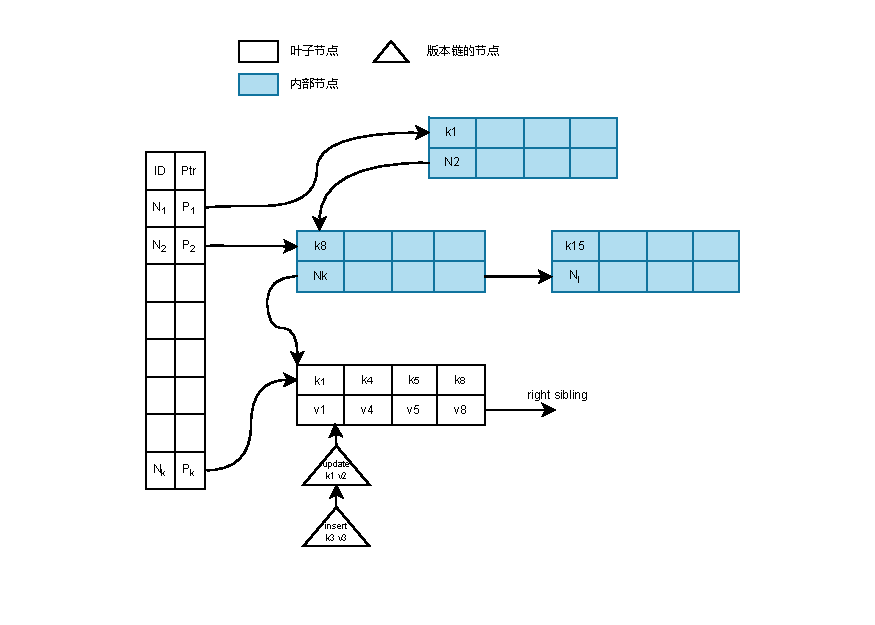
\includegraphics[width=0.9\textwidth]{bwtree.pdf}
  \caption{Bw-Tree的设计概图}
  \label{fig:bwtree}
\end{figure}

Hekaton\cite{larson2011high} 是微软 SQLServer 专门针对 OLTP 应用场景进行优化的数据库引擎,
其索引实现基于 Bw-Tree。Bw-Tree 是一种无需使用任何锁同步的 B+Tree,其主要设计思想如下:

Mapping Table(映射表) 映射表存储内存页的ID与其对应的物理内存地址,
使得线程可以通过访问映射表找到需要方位的内存地址,映射表通过CAS操作来更新。
所有操作不直接修改节点,任何的更新操作都会生成新的数据并且通过指针来指向需要被更新的节点;
新生成的数据所导致的元数据的修改,比如修改映射表都通过 CAS 完成。
垃圾回收机制,Bw-Tree 通过不断新增数据的方式避免直接修改树节点,
在树不断更新的过程中,我们需要对之前旧的数据进行回收,避免版本链的无尽增长降低查询效率。
因此 Bw-Tree 实现了基于 Epoch 的垃圾回收机制:
当一个线程想保护一个它正在使用但是将会被回收的对象,例如检索的时候,
访问了一个内存页,就把当前线程加入 Epoch,当这个线程完成检索页面的操作后,就会退出 Epoch。
通常一个线程在一个epoch的时间间隔内完成一次操作,例如检索。
在线程成功加入 Epoch 的时候,可能会看到将要被释放的老版本的对象,
但不可能看到已经在前一个 Epoch 中释放的对象,因为其在当前 Epoch 中的操作并不依赖上一个 Epoch 中的数据。
因此,一旦所有的线程成功加入Epoch 并完成操作然后退出这个Epoch,回收该 Epoch 中的所有对象是安全的。
由于维护了映射表,和新增数据链,因此树结构调整相对复杂,
不仅仅要调整树,切要保证树结构和映射表之间的关系。

尽管实现非常复杂,Bw-Tree 作为无锁的数据库索引树,有如下优势:
\begin{itemize}
\item No Latch: 实现无锁数据结构十分困难,Bw-Tree 在多线程场景下没有引入任何的latch,
只使用 CAS 指令保证线程同步,因此多核的扩展性优于普通用锁同步的B+Tree。

\item CPU Cache: 由于不直接修改节点而是追加修改补丁,
因此 CPU 缓存不会应为更新数据而失效,因此可以显著提高 CPU 缓存命中率。
微软论文中的数据表明,百分之九十的读操作数据来自 CPU L1/L2 缓存。
\end{itemize}

综上也可以看出Bw-Tree尽可能的不原地修改结构,使用CAS避免悲观锁导致的低扩展性。我们在设计实现乐观级联锁的ART索引时主要参考
Bw-Tree中的去中心化的垃圾回收机制的实现。

\section{Masstree}
\subsection{Masstree 简介}
2012年发表的论文 Cache craftiness for fast multicore key-value storage 提出了 Masstree,其特点如下:

可以理解为B+ Tree 和 Radix Tree 的混合体,即将键切分成多个部分,每个部分为一个节点;
每个节点内部又是一个 B+ Tree,兼顾空间和性能。
Masstree将变长键划分成多个固长部分,每个固长部分可以通过int类型表示,而不是char类型。
由于处理器处理int类型比较操作的速度远远快于char数组的比较,
因此Masstree通过int类型的比较进一步加速了查找过程。固定长度可以设置为 CPU 缓存行长度,以增加 CPU 缓存效率。
每个节点是一个 B+ Tree,因此 CPU 在查询的时候可以将节点所代表的B+ Tree 加载到 CPU 缓存中,
以增加 CPU 缓存命中率\cite{binna2018hot}。

\begin{figure}[h]
  \centering
  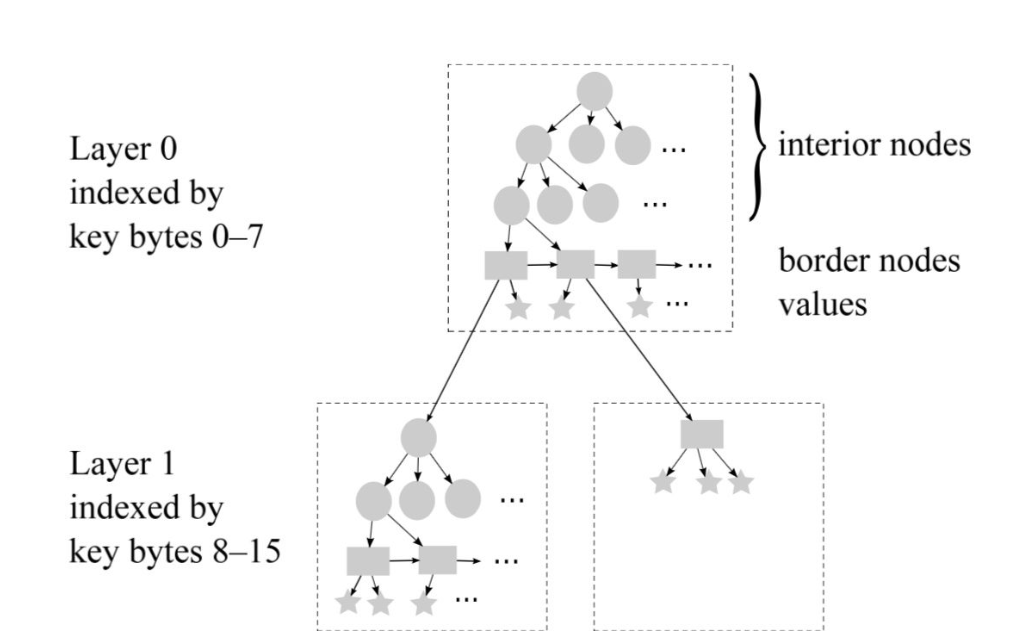
\includegraphics[width=0.9\textwidth]{masstree.png}
  \caption{MassTree的设计概图}
  \label{fig:masstree}
\end{figure}

\subsection{Masstree 并发控制}
MassTree使用细粒度的锁和乐观并发控制来保证高并发。
读并不阻塞写;
写流程要保证并发的读线程不会读到不一致的中间状态;
写写之间用自旋锁互斥。
读操作对比读前和读后记录的"版本号"是否变化或是否被标识为“dirty”或是否被加了写锁,
这些迹象说明有写线程在并发修改记录,读操作重试。

\section{小结}

我们简单介绍了以上几种数据库索引类型以及他们各自的并发控制算法,从上面的索引类型我们可以发现,在内存数据库中
大家普遍采用的是了乐观并发控制,同时这几种数据库都聚焦于提高Cache命中率,避免读操作导致Cache失效,而需要去内存中再读取
数据。同时因为采用乐观并发控制,还需要对于待删除的内存进行管理,不可以立即将内存回收,基本上都是采用的基于Epoch的垃圾回收机制。
这给我们设计和实现基于乐观级联锁的ART索引提供了很大的启发和实现原型。

我们在数据库索引选型时考虑采用ART索引,并使用乐观级联锁处理ART索引的并发控制。我们使用ART索引主要是作为二级索引,主要使用场景是
作为IPTables的索引表。因此我们的ART索引除了提供基本的查询,插入,删除,范围查询接口外,也需要做到对最长前缀匹配的支持。
此外数据库中创建和删除索引等基本的DDL操作也包含在本文的范畴内。

目前商用的DBMS并不是特地为多核CPU而设计,随着核心数的增多,并发控制变得越来越困难,多核并发带来的收益会越来越小,造成实际上的
资源浪费。所以我们主要关注索引结构及其并发算法的可扩展性,这也是为了之后,可以将部分对索引的操作卸载到硬件上所做的必要的预研。

 % 相关内存索引
% !TeX root = ../main.tex

\chapter{基于乐观级联锁的模块设计}

索引模块是数据库存储管理模块的重要组成部分。索引模块的设计,同时也需要考虑数据库中整体存储管理模块的设计与实现,
做到二者无缝衔接。接下来的一章,我们将着重介绍基于乐观级联锁的索引模块的设计,同时我们还会介绍当前系统的存储模块与索引
模块交互的部分。

我们将本章分为6个小节逐步介绍ART索引模块。2.1小节主要介绍ART的底层数据结构设计,2.2小节重点介绍了如何基于乐观锁的并发控制
2.3小节介绍了数据库索引模块的内存管理机制,2.4小节介绍索引的操作算法设计,2.5小节主要介绍如何针对不同的数据类型设计相应的Key,
2.6小节介绍了创建和删除索引所需要的事务机制支持,2.7小节介绍了数据库内存表的组织方式,2.8小节对本章内容进行了小结。

\section{ART的底层数据结构}

ART(Adaptive Radix Tree)意为节点可伸缩的前缀树,下面我们将重点介绍这一数据结构的详细设计

\subsection{ART索引节点的头部设计}

\begin{figure}[h]
  \centering
  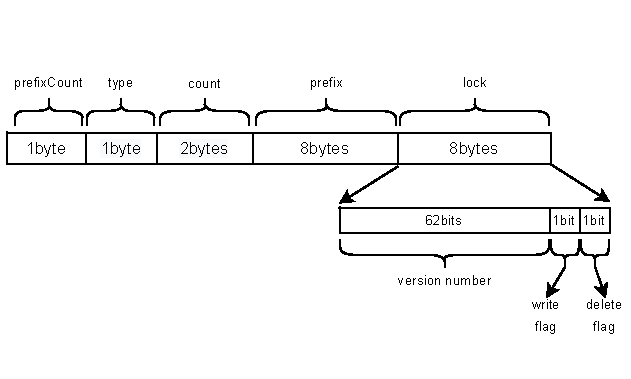
\includegraphics[width=0.9\textwidth]{art-node-design.pdf}
  \caption{ART索引节点的结构图}
  \label{fig:art-node-design}
\end{figure}

与一般前缀树相比,ART最特殊的地方在于内部节点的大小可以根据节点的实际容量而改变。因此我们也需要额外的信息来维护
节点的信息。ART节点分为4种类型,每一种类型的节点都包含一个通用的头部,如下图所示:prefixCount表示公共前缀的长度;
count表示当前节点的子节点个数;optimistic lock用作下文中即将介绍的并发控制机制, 64位原子变量,最后两位分别作为
标记删除和标记修改位;此外由于本索引还需要支持最长前缀匹配,即可能出现某个键值可能是已有键值的前缀,所以还需要加入
isPrefix 和 PrefixSlot 这两个变量分别为标记当前节点是否包含一个额外的子节点和存储子节点的槽位。公共前缀的目的在于
压缩字典树的深度,防止字典树深度过大,造成内存的开销以及访问开销。

\subsection{ART索引各个节点结构定义}

\begin{figure}[h]
  \centering
  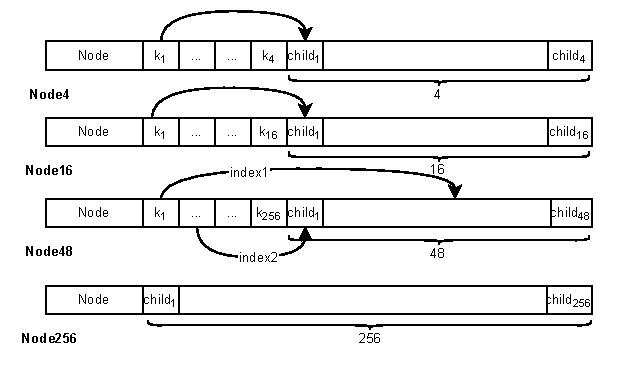
\includegraphics[width=0.9\textwidth]{art-nodes-design.pdf}
  \caption{ART所有类型索引节点的结构图}
  \label{fig:art-nodes-design}
\end{figure}

上面我们已经介绍了所有类型的ART节点都包含的公共头部,下面我们依次介绍每一种节点的设计以及针对每一种节点的优化。
我们按照节点可存储子节点的个数规定四种类型的索引内部节点。依次标记为Node4、Node16、Node48、Node256。下图定义了
四种节点的内存布局。Node4节点keys数组存储键值,children数组存储子节点指针,keys和children一一对应,且keys为
有序数组;Node16节点节点布局和Node4相同只是子节点个数为16,不同的是由于存储个数较多,所以针对节点查询可以利用
SIMD同时比较16个key上的值,后面实现章节会详细说明;Node48节点存储的就是256个key和48个子节点槽位,keys中存储
的是对应在children的索引,即keys[i]与children[keys[i]]对应,无效的keys中存储48即可。Node256节点就是最常规的
前缀树索引的节点。
此外,我们还需要说明所有children中存储的都是指向子节点的指针,由于索引的应用场景为内存数据库,因此使用指针即可
访问对应的子节点。但是同时也引入了一个问题,即如何区分叶子节点?这里我们考虑到实际虚拟内存寻址也仅仅使用低48位内存
地址,所以需要将叶子节点指针的最高位标记为1。

由于本系统需要支持lpm(最长前缀匹配),因此需要针对此需求特殊设计一种ART索引。
因为前缀树本身并不允许一个key是另一个key的前缀,所以可以修改节点的定义,在节点的头部加入一个标记位,
标记当前节点是否作为一个叶节点。
而对于插入删除等索引操作部分的优化,则在接下来的章节部分做出说明。

\section{基于乐观级联锁的并发控制机制}
本论文采用乐观锁来实现ART索引的并发控制。在基于乐观锁的ART索引并发机制中,我们重点关注下面的两个问题:

(1)应当避免某个写操作持有写锁导致其他读写操作多次从根节点重新操作,造成CPU资源的浪费,因此可以在读写操作中加入判断条件即restart次数大于阈值时进程睡眠,让出CPU资源,避免进程被CPU反复无效调度。

(2)同一个进程至多只会同时持有两把写锁,即当前结点和父亲结点。且申请顺序为先申请父亲结点再申请当前结点。且当修改结点的操作完成后应立即释放持有的写锁。索引的插入删除等过程后面具有具体的论述。

我们在每个ART索引节点中都使用一个64位的原子变量作为乐观锁。
当对索引进行操作时,总是先从根节点开始向下访问。
初始访问索引节点时总是先读取该结点元信息中原子变量(optimistic lock)获得结点的版本号。
对于查询操作,读取结点的数据之后,总是检查当前结点的版本号是否与初始访问时一致,若不一致则重新从根节点进行上述操作。
若一致方可继续向下访问。对于更改操作,仍是需要检查版本号一致性,
再对该结点升级为写锁(即是对原子变量加2,解锁时仍是对原子变量加2,所以其对应的版本号便增加了1),
若加锁失败则重新从根节点进行上述操作。当我们不再需要这个结点时,将删除位置1 。
需要注意的是当结点的lock或者delete位被标记时,
任何检查结点原子变量一致性的操作都必须返回失败,程序重新回到根节点开始操作。

上述内容介绍了基于乐观级联的并发控制机制,上述内容中有一个显而易见的问题就是,因为采取了乐观锁这种机制,会导致读进程被反复的restart。
由于每次操作都被restart,会导致这个线程一直占用着cpu重复这样子的操作,而造成资源浪费和后续的操作得不到执行。如何避免这个问题,通常有两种方式,
第一,对于频繁被restart之后,直接给索引加锁,以插入的方式给每个节点加上写锁。这会导致实际编码时存在两套编码,同时这也不能缓解实际频繁重启的问题。
第二,将线程挂起,使用类似于网络通信中规避算法,当重启次数超过阈值,挂起进程。随着重启次数增多,挂起时间越长,规避的时间也就越长,这会缓解CPU操作的负载,
但是也可能导致读线程始终得不到执行。本文中使用的是第二种避让方式,当重启次数过多,直接挂起线程。

\section{内存管理模块}
本小节主要介绍ART索引的内存管理模块,由于ART在插入删除等操作的过程中结构一直在变化,随着节点中子节点个数的增加或减少节点也会随着膨胀或者缩减为另一类型的节点。
旧的节点应当被回收,ART作者提出的GC操作,分为集中式GC和分布式GC两种,集中式GC会导致GC模块成为系统的瓶颈,
而分布式GC 编程复杂,且节点内存申请和回收都会导致一次系统调用造成开销。我们考虑到旧的节点被回收,
但是插入操作仍需要申请新的节点,这仍然会导致一次系统调用,造成开销,因此提出用无锁队列回收需要删除的节点,
暂时并不归还操作系统。若回收的垃圾节点过多,再统一归还操作系统。

\subsection{无锁队列设计}

\begin{figure}[h]
  \centering
  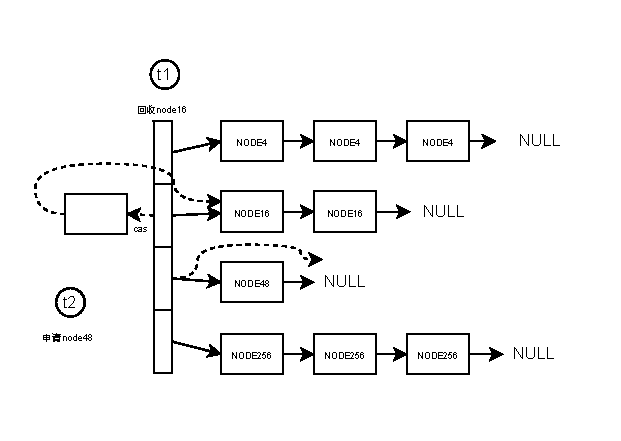
\includegraphics[width=0.6\textwidth]{art-obj-pool.pdf}
  \caption{基于无锁队列的垃圾回收}
  \label{fig:art-obj-pool}
\end{figure}

索引内存模块的空闲队列结构如上图,通常情况下,索引申请新的结点总是先从内存管理
器获取,如果内存管理器中该节点类型的空闲链表上没有空闲结点就使用 malloc 从系统申请。
当结点被标记删除时,不是立即归还给操作系统,而是将结点中 delete flag 标记为 1,同时将结
点插入到空闲队列的队头,这一步可以使用C++ 11 中的compare\_exchange\_weak 或
compare\_exchange\_strong 实现一个无锁的队列。
将一个被标记删除的空闲 Node16 结点插入空闲链表的头部。
不立即将内存归还操作系统的原因在于当前结点被标记删除后,该结点可能还被其他读进程
所占用,其他读进程仍会继续访问该节点中数据。我们将该结点标记删除后放入空闲链表,读进
程获取结点数据之后需要验证版本号,便会发现该节点已被删除需要重新从根节点进行访问。

\subsection{基于epoch的垃圾回收机制}

上述的内存管理机制适用与当前系统使用预先分配内存的方式管理内存空间。若需要及时将不用的内存归还操作系统的话,也可以通过后台的垃圾回收线程
固定回收无锁链表里的内存块,但这一操作存在风险,因为最先回收的内存总是最新标记删除的,而且随着并发度提升,无锁链表也会成为系统的瓶颈。
因此需要提升并发度,则不能使用上述内存管理机制。下面我们介绍两种基于Epoch的垃圾内存回收机制,这两种机制也是Bw-Tree作者提出的管理Bw-tree内存的机制。

\begin{figure}[h]
  \centering
  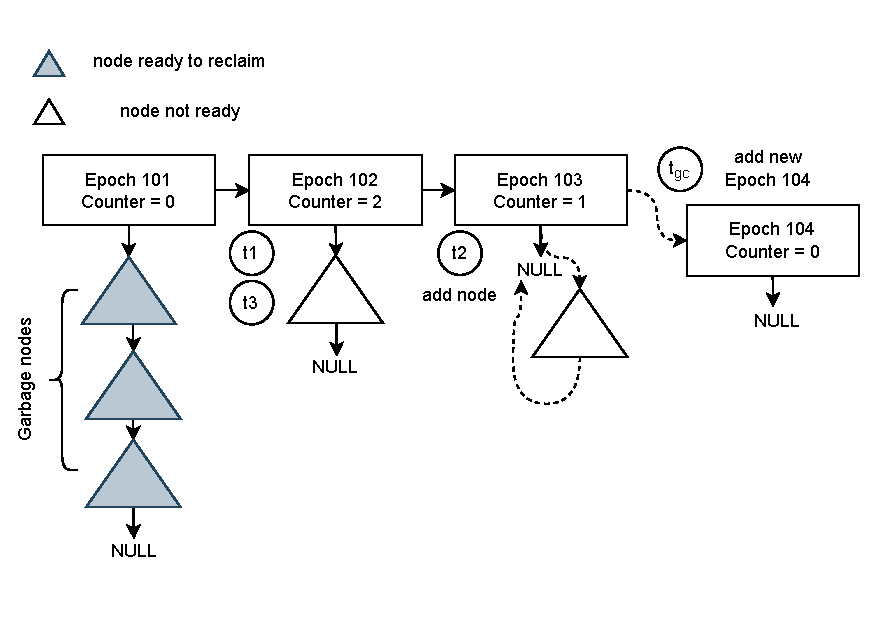
\includegraphics[width=0.7\textwidth]{art-gc-center.pdf}
  \caption{基于Epoch的中心化垃圾回收机制}
  \label{fig:art-gc-center}
\end{figure}

首先是基于Epoch的中心化的垃圾回收机制,索引维护一条全局的epoch对象链表。
后台垃圾回收线程每隔一段时间(40ms),会在链表的尾部添加一个新的epoch结构。
每个线程在访问索引内部数据结构之前,需要在当前的epoche结构中注册自己的操作,当操作完成的时候,将自己从注册过的epoch中移除
任何被标记为删除的对象都会被加入当前epoch的垃圾回收链表里。当所有的线程都离开了这个epoch,索引的垃圾回收线程会将这个epoch中
所有被标记为删除的结构回收。

上图中展示了这种中心化的垃圾回收机制。图中分别有三个工作线程和一个后台运行的垃圾回收线程。在这张图中,t2线程将一个新的节点加入
epoch103,同时垃圾回收线程新增了一个epoch104。而epoch101中的引用计数降低为0。垃圾回收线程将epoch101中所有记录的节点回收。
将其内存释放。这种垃圾回收机制的扩展性非常差,不适合作为多核多线程应用场景下使用。因为这会面临多个工作线程同时进入epoch中,同时
增加引用计数,造成资源争用。因此这会成为系统的性能瓶颈。所以以下我们讨论open-bwtree中提到另一种基于epoch的去中心化垃圾回收机制。

\begin{figure}[h]
  \centering
  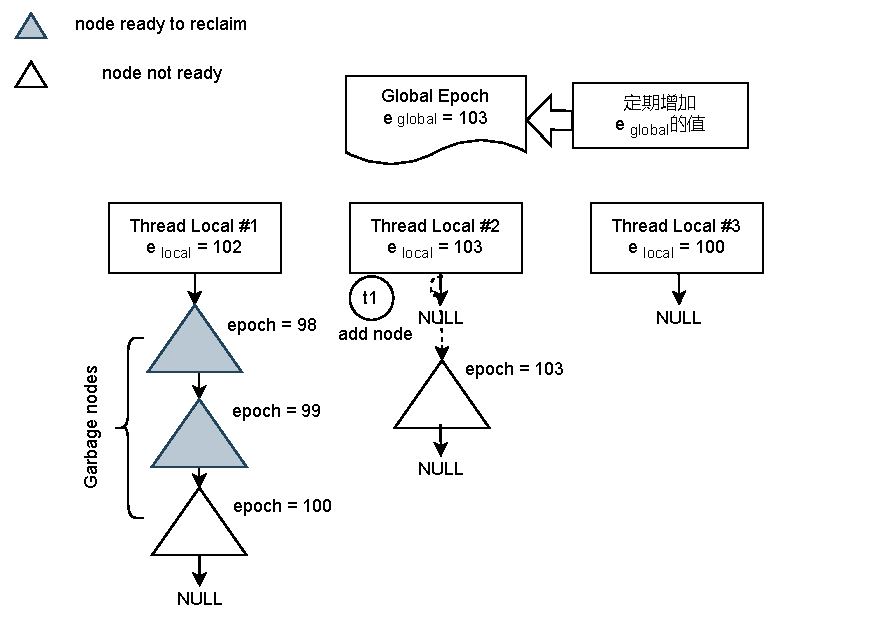
\includegraphics[width=0.7\textwidth]{art-gc-decenter.pdf}
  \caption{基于Epoch的去中心化垃圾回收机制}
  \label{fig:art-gc-decenter}
\end{figure}


上图这种去中心化的垃圾回收机制可以避免线程将数据写入到全局的内存中,从而避免多个线程并发操作导致争用问题。
下面我们详细阐述一下关于去中心化垃圾回收机制的设计。索引模块维护一个全局的epoch,每个工作线程也会维护一个本地的epoch和一个指针链表,
链表中的元素指向的是线程标记删除的对象。
还是继续使用以下的例子举例。t1作为唯一的工作线程,他将一个垃圾节点放入自己维护的链表中,并且将该节点标记为当前的epoch103。
在某个操作开始之前,线程总是先去全局的epoch拷贝一份标记删除的链表备份到自己私有的epoch中。
在进行任何操作之前,工作线程总是先从全局的epoch中读取最新的epoch存入自己的私有epoch中,此后如果该工作线程需要删除某个节点,
则将该节点标记为删除,同时将该节点标记上工作线程当前的epoch并放入自己私有的待删除链表中。

当该工作线程的工作结束之后,线程遍历所有其他工作线程的本地epoch找出最小的epoch,同时搜索本地私有链表中需要删除节点上标记小于该epoch的节点,将内存回收给操作系统。
而为了推进这个操作的可持续性,DBMS会维护一个后台线程定期增加全局的epoch。

综合以上的论述,详细阐述了如何设计基于epoch的去中心化的垃圾回收模块。其目的还是在于提高cache的命中率,期望通过读而不是写的方式可以完成线程间的同步。
使用ThreadLocal这一机制,避免了使用锁或者其他同步机制。为了方便进行编码,后面实现章节我们将借助于Intel现有的ThreadLocal库来进行操作。
后面的实现章节我们会在索引模块中分别实现两种垃圾回收机制。在实验章节,我们会对比这两种垃圾回收机制,在各种使用场景下的性能对比,
最后我们选择在不同的场景下,应当是使用不同类型的垃圾回收机制。

\section{索引主要操作流程}
这里我们介绍本章的重点就是对ART索引的并发控制,我们需要注意这里介绍的只是对ART这一数据结构的并发控制,
即同时对索引进行读写操作并不会影响数据的正确性,
关于数据库中事务的并发控制,我们将在下面小节作简单介绍,如何应用当前数据库中的事务机制做到对索引的DDL操作和DML操作也可以并发操作而不影响正确性。、
在本小节中我们主要介绍索引的查找,插入,删除,范围查找。

\subsection{查询流程}
ART索引的查询流程如上图所示,查询过程是一个只读的过程因此并不涉及到内存的申请或者释放。具体的查询流程为:

1.初始化操作:将根节点作为当作当前节点。

2.读取当前节点的版本号。

3.比较当前节点的前缀是否与需要查询的key匹配,如果匹配进入下一步骤4,如果不匹配则结束查询,返回空值。

4.当前缀匹配时,需要读取对应的槽位上是否包含子节点,如果包含子节点且为叶节点则返回其值;
若不为叶节点,则转到步骤5。

5.校验此时版本号与步骤2中的版本号是否一致,若一致说明此期间该节点没有被修改。
将非叶子节点指针读取出来赋值到当前的节点,回到步骤2进行操作。由于树形结构的深度有限,
读操作总是会读取到值或者没有匹配的值而结束这一循环。

\subsection{插入流程}
ART 索引的插入流程如上图所示,插入流程涉及到节点的扩容和新增,因此需要与内存模块交互,同时因为需要有扩容操作,涉及到将
旧的节点标记删除。

\paragraph{插入流程}
1.初始化操作:将当前节点置为空指针,将next节点置为根节点。

2.将当前节点赋值给父亲节点,next节点赋值给当前节点,读取当前节点的版本号。

3.比较当前节点的前缀是否与需要查询的key匹配,如果匹配进入第4步,如果不匹配则进入第6步。

4.验证当前节点的版本号是否与第2步读取到的一致,若一致则进入第5步,若不一致则返回第1步。

5.检查对应的槽位上是否有子节点,若含有子节点则将对应槽位上的子节点指针赋值给next指针,返回第2步,重复流程。
若对应槽位上子节点指针为空则升级当前节点和父亲节点的锁为写锁,若升级锁成功则插入新的节点;若升级锁失败,返回第1步重试。
在这里需要注意的是插入可能会导致节点类型升级,所以也需要升级父亲节点的锁为写锁。

6.当前节点的前缀与插入的key不匹配。首先获取父节点的锁,然后获取当前节点的写锁。
若有一个失败,则返回第1步重试。再次取出取出两者的公共部分,申请一个新的Node4类型的节点,
将当前节点和需要插入的节点分别插入其中对应位置。将父结点中对应的子节点指针修改为新申请的Node4节点的地址,完成插入流程。

\subsection{范围查询流程}
范围查询是索引中经常使用的一种查询方式,比如select * form tb where idx < 1000 and idx > 200,
且idx字段为索引字段。ART索引的范围查询流程如下所示。

1.初始化操作:将根节点作为当作当前节点。

2.读取当前节点的版本号。

3.比较当前节点的前缀与startKey和endKey的大小关系,若startKey大于当前前缀或者endKey小于当前前缀,说明不存在有效的结果。
此时应当验证版本号,若与步骤2中的一致,返回空集;若不一致,则返回第一步中的根节点重新查找。

4. 若当前的前缀恰好在闭区间startKey和endKey之间(此处应当是严格小于endKey[level],严格大于startKey[level],level表示此时在键值中的位置),
验证版本号若一致,则将当前节点下所有的叶子节点存储Tid加入结果集,返回结果;若不一致,返回第一步重新开始查询。
若前缀恰好可以完全匹配当前的区间要求,则读取当前节点上的所有满足闭区间[startKey[level+1], endKey[level+1]]的子节点指针。
针对边界值,使用递归进行查询,以区间的起始位置举例,查询的范围变为[startKey, 无穷大值],同理针对区间的结束位置,查询范围变成了
[无穷小值, endKey]。因为ART树的内部节点键值的取值范围为0至255,因此这里的无穷大,无穷小对应的分别就是全部字节皆为255和0的
键值。而针对非边界的子节点指针,查询的方式类似于前面的前缀恰好严格落在查询区间中的方式。
最终我们返回的是三者的并集。

\subsection{删除流程}
删除流程大致与插入流程类似,区别在于删除节点可能会导致节点收缩,当子节点的个数低于阈值时,需要将容量较高的节点缩减为下一级
容量的节点,这里我们需要修改父节点中对应的指向子节点的指针,同时需要将原来节点中的子节点拷贝到新的节点中,并将原节点标记删除。
以下为详细的流程设计:
\paragraph{删除流程}
1.将根节点作为当前节点。

2.读取当前节点的版本号。

3.比较当前节点的前缀是否与需要查询的key匹配,如果匹配进入第4步,如果不匹配则直接返回。

4.验证当前节点的版本号是否与第2步一致,若一致则进入第5步,若不一致则返回第1步。

5.检查对应的槽位上子节点是否为空指针,若对应的子节点不为空且不是叶子节点则将当前节点替代为子节点,返回第2步,继续向下搜索。
若对应的子节点指针不为空且为叶子节点则升级当前的节点与父亲节点的锁等级,删除对应的叶子节点。这里升级父亲节点的锁等级的目的在于
当前节点删除一个子节点指针之后会不满足当前节点类型的最低子节点个数的要求。因此这里需要申请更小类型的索引节点,并将父亲节点
中的对应子节点指针修改为新申请的节点。

\section{不同类型数据的键值设计}
我们知道在数据库系统中存在着许多不同的种类,在类型上大体可以分为变长和定长,索引需要向外提供范围查询功能,因此实际上
存储的数据应当是有序的,这样会方便我们进行范围查询。
而由于ART树的特殊性,每个节点只存储部分索引的字段,所以合理的安排索引的顺序就显得非常重要了。
由于前缀树的设计,我们需要对不同类型的数据做出适当的变换以适应前缀树的存储方式。
以下我们重点介绍int/uint, float/double,String,复合的key。

\subsection{int/uint的存储结构设计}
对于unsigned类型其对应的二进制类型仍具有既定的顺序,但是我们仍然需要考虑到大小端的问题。
因此对于小端系统,我们需要将字节序反转以保证结果是有序的。而如何判断系统属于大端还是小端系统,可以在系统中定义相关的宏,
编译器根据指定平台的编译出相应的代码。

而对于signed类型,则需要重新排序,因为负数在计算机中按照补码存储,
一个b位的整数x可以通过反转符号位转换为正常的顺序(x XOR $2^b$-1),变换后有符号数就可以按照无符号树的顺序进行比较,
随后就可以作为正常的无符号进行存储。

\subsection{float/double的存储结构设计}
首先对于IEEE754类型的浮点数,可以优先根据符号位将其区分为整数和负数,
其次可以将其分为规格化的值,非规格化的值,NaN,无穷大/小,0。总计十种数值。
他们彼此之间是没有交集的。因此只需要将阶码,尾数转换为对应的无符号数处理即可

以double类型举例,考虑其13位的阶码和52位的尾数,分别使用2字节和9字节存储。最高为符号,因此这样的话root节点只需要作为
一个Node4类型的节点存储两个key指向的孩子节点。

\subsection{string的存储结构设计}
对于string类型的处理分为两种,一种较为简单针对定长的string类型,我们可以简单的将其对齐到指定的字节数(128bytes,256bytes,512bytes)。对于空出来的位数可以直接填0。
对于不定长的string类型,这种数据类型主要的使用场景是支持LPM(最长前缀匹配),
这需要我们修改原本的数据结构,即在node header中加入一个判断条件支持多增加的这一对(key/value),当进行前缀比较时,需要注意这一点,
因为原始的ART中是不存在前缀特征的键值的,而这里加入前缀特征之后,每一个节点的孩子节点的容量都会增加1,而且为了支持最长前缀匹配,当搜索key时
需要作出特殊处理。这在后续的支持LPM匹配的查询处做详细说明。
通常情况下我们所存储的key均为定长数据,因此不会产生这种一个键值是另一个键值的前缀的场景。

\subsection{compound key的存储结构设计}
对于复合类型的key,通常情况下,生成索引部分需要传入组合键值的相应参数,IndexBuilder根据参数生成相应的索引结构。
因此只需要在传入参数时,根据上述介绍的规则逐个转换,选择合适大小的索引类型生成即可。

我们需要注意的是本索引并不允许两个重名的字段出现,即需要索引的字段应该是全局唯一的,但是实际上许多字段并不能做到全局唯一,
因此,我们需要在判断字段是否相同时,加入该字段的唯一主键,这个主键可以是记录的TID。以上便可以做到全局索引到唯一的一条记录。

\section{事务机制}
上述介绍的索引模块中引入的并发控制机制仅仅是针对该数据结构的并发控制,全部为DML操作,还有一类比较特殊的操作例如
create/drop index操作。

针对创建索引的操作,索引模块主要接口为根据keySchema创建相应的索引,这里主要是根据keySchema确定ART索引中键值的长度。
根据以上小节提到的针对不同数据类型所需要作出的更改。

针对需要删除索引的操作,这里有两个地方需要注意。一个是当索引模块需要删除该索引时,可能还有其他事务的进程在读取该索引,
所以我们并不能直接删除索引,而是利用一种叫做DAF事务框架的方式,作延迟删除。详细的如何延迟删除在下一小节讲解。
另一个需要注意的地方是需要删除所有索引的内存,如果索引采取的预先分配内存的方式,那么直接回收内存即可。如果采用的
是基于Epoch的垃圾回收机制,则需要从根节点开始,以类似于后序遍历的方式,逐个回收节点内存,由于采用的是去中心化的垃圾回收机制。
随着最后一个操作结束,如果此时操作退出时没有能够回收已经标记删除的内存,那这块内存会一直保留着。
因此基于Epoch的垃圾回收机制还需要注意在清理对象时,回收掉没能立即被回收的内存块。

\subsection{DAF的基本结构设计}
DAF事务框架(Deferred Action Framework)核心在于
如何将事务性的修改(删除索引中的一条记录)和非事务性的修改(删除索引)结合。
框架的核心在于将所有对实际物理结构上的操作都注册为一个action,
数据库系统针对不同的命令会执行对应的action, 但是这些action真正的执行需要等到系统安全为止。
直到该版本不再被当前活动的事务可见时管理器就会删除这个版本。

\subsection{DAF事务框架}

\begin{figure}[h]
  \centering
  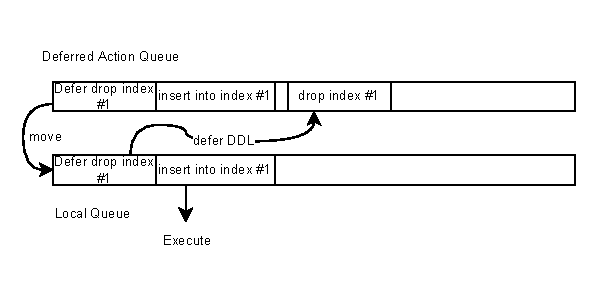
\includegraphics[width=0.7\textwidth]{daf.pdf}
  \caption{DAF 延迟删除}
  \label{fig:daf}
\end{figure}

由于DAF事务框架的设计规定,我们在整个系统设计一个DAF Manager,
他负责管理事务延期执行的行为。主要设计思路是维护一个队列,队列里的元素为Deferred Action,
而Deferred Action则为对应的一个个动作。如上图,当索引需要删除时,将这个删除索引的操作,注册到
DAF Manager中,这个操作实际上注册是延迟删除索引的操作,因此当DAF Manager 执行以下队列的操作时,尽管删除索引的
操作在对索引执行插入操作之前,但是实际上,DAF Manager只会将该drop index 操作再次注册进队列中,等待下次执行队列的机会。
而且在执行Deferred Action时可以执行并发操作,因为此时所有需要删除的记录都是对当前事务不可见的。

这里的事务框架是系统中已有的事务框架,我们这里只是简单介绍其与索引模块相关的操作。

\section{底层存储机制设计}
上述章节已经介绍了索引设计和如何将索引引入数据库中。
下面我们再介绍一下底层存储模块即表存储设计,
由于本索引应用于内存数据库即所有的数据都存储在内存上因此没有传统数据库中的buffer pool的概念,
但是我们仍然需要建立对内存块的维护,并且设计新的内存存储系统。

\subsection{底层存储组织格式}
传统的数据库往往根据其主要的使用场景将其分为OLAP和OLTP,
针对OLTP数据库来说,其往往会采用行式来组织数据,
而OLAP数据库会采用列式组织数据,这两种数据组织方式各有其优缺点。
而我们采取的是行列混存方式,同时还可以引入冷热数据分开存储的方式,
将冷数据转换为Arrow的纯列式存储,不仅方便数据后期的分析查询,还可以提供通用接口供其他应用调用。

\subsection{PAX行列混存格式设计}

\begin{figure}[h]
  \centering
  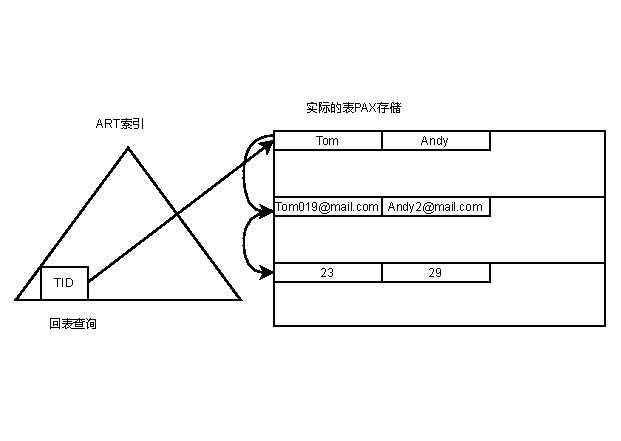
\includegraphics[width=0.7\textwidth]{art-table-pax.pdf}
  \caption{PAX行列混存格式}
  \label{fig:art-table-pax}
\end{figure}

行列混存格式,即将整个数据分成合适大小的block,在block之间采用行存方式组织数据,
但是在block内部采用列存。block内部根据该表的所存储记录的metadata,将每一个block划分为多个miniblock
每个miniblock的大小根据metaData计算出来,因此所有的miniblock的大小在插入数据之前就已经确认了。所以实际block的存储
记录中不可以含有变长记录。这点可以通过超过指定长度的变长数据就通过指针方式存储。
而且由于是内存数据库,因此每个block可以根据指针直接访问。每个block内部的数据组织格式如下图所示。
这里主要是提出对变长信息的优化,由系统维护一个var entry 管理器,超过16字节的变量就由varlen负责存储。
采用前8字节为长度,后8字节为变量的地址。即可寻址到具体的变长变量。
同时这里也可以做到一个如果实际存储的字段的基数较低,可以部分存储字段,而不用完全存储。
通过低基数优化还可以同时优化字段作为聚合字段时的开销。
上文中提到ART索引,作为系统中的辅助索引,其每一个叶子节点均指向实际的内存地址(即图中所示的version ptr)。
由于正常的linux系统中,虚拟地址只需要前48位,因此我们可以将最高位置为1的方式,来区分叶子节点和实际的虚拟地址空间。

这样,我们在索引的叶子节点中只需要存储TupleId,即存储一个64位的地址。通过这个地址,再去内存的表中读取相应的记录。

\subsection{Apache Arrow存储格式}
由于系统中存在两种数据组织格式,冷数据以Apache Arrow\cite{ahmad2020arrowsam}格式组织,方便其他应用直接获取。
Apache Arrow 是一种跨平台跨语言的内存列式数据组织格式。
在Apache出现之前,每个系统之间互相传输数据都需要经过序列化和反序列化,在系统数据量较大的情况下,大量计算资源消耗在上面,这无疑造成了系统的开销。
Arrow数据组织上严格按照字节对齐,最大化利用硬件带来的向量化和SIMD加速。其将数据分为两类,定长和变长数据类型,并使用Array表示。定长Array包括
数据类型,长度,空值个数,空值位图,按字节组织的列数据。
变长与定长组织方式类似,但是会多一个数据偏移字段,以帮助数据快速定位和计算长度。

因此内存索引中如何索引这些按照Arrow格式组织的冷数据。
可以建立一个对于冷数据的管理器,根据TID的标记到这个管理器中查询对应的记录。由于Arrow格式本身
也可以持久化到磁盘中,因此如果系统开启了冷热数据分区的话。
对于冷数据的索引就会退化为面向磁盘的数据库索引,因此已经不再适合当前的索引类型。所以本文只讨论
所有需要索引的记录均存储在内存中。

总的来说,目前ART索引只适合索引那些存储在内存上的数据,如果涉及到需要与磁盘交互的部分,那么索引的很多设计思路就失效了。
因此ART索引只适合作为内存数据库索引而被使用。

\section{本章小结}
本章先介绍了基于乐观锁的ART的诞生背景以及明确索引设计的目标,对索引的各个部分的设计和流程进行了简要介绍。
首先是索引node中各个参数的内存分布,以及如何基于原子变量实现乐观锁,
其次介绍了级联锁即每个并发操作只会同时拥有两把锁。
针对并发操作中可能产生的内存回收问题,设计无锁队列回收内存,并重复使用该内存,降低了系统调用的开销。但是以上这种方式仅适用于
预先分配内存的情况。针对不预先分配内存,实时申请释放内存的系统,采用基于Epoch的垃圾回收机制。
然后我们逐个介绍了索引的点查询,删除,插入,范围查询等流程。
最后两小节中,我们介绍如何将数据库索引的DDL操作与DML操作都融入数据库的事务系统中,但这部分并不是本文讨论的重点。
此外我们还介绍了实际数据库系统中表的存储结构采用PAX的存储方式,通过TupleID 访问一条记录需要跨过多个miniBlock,
因此这里我们就不再对索引进行路径压缩,在路径上保留完整的key,只通过公共前缀的方式进行数据压缩。
 % art 索引模块设计
% !TeX root = ../main.tex

\chapter{索引模块的实现}

之前的章节中我们着重介绍了如何设计索引的各个组成部分,接下来的一章中,我们将探讨如何实现这一索引.

\section{索引节点的底层存储实现}

以下定义索引节点的结构体,如图所示所有类型的索引节点都包含一个仅有头部数据的节点类Node。

\begin{figure}[h]
  \centering
  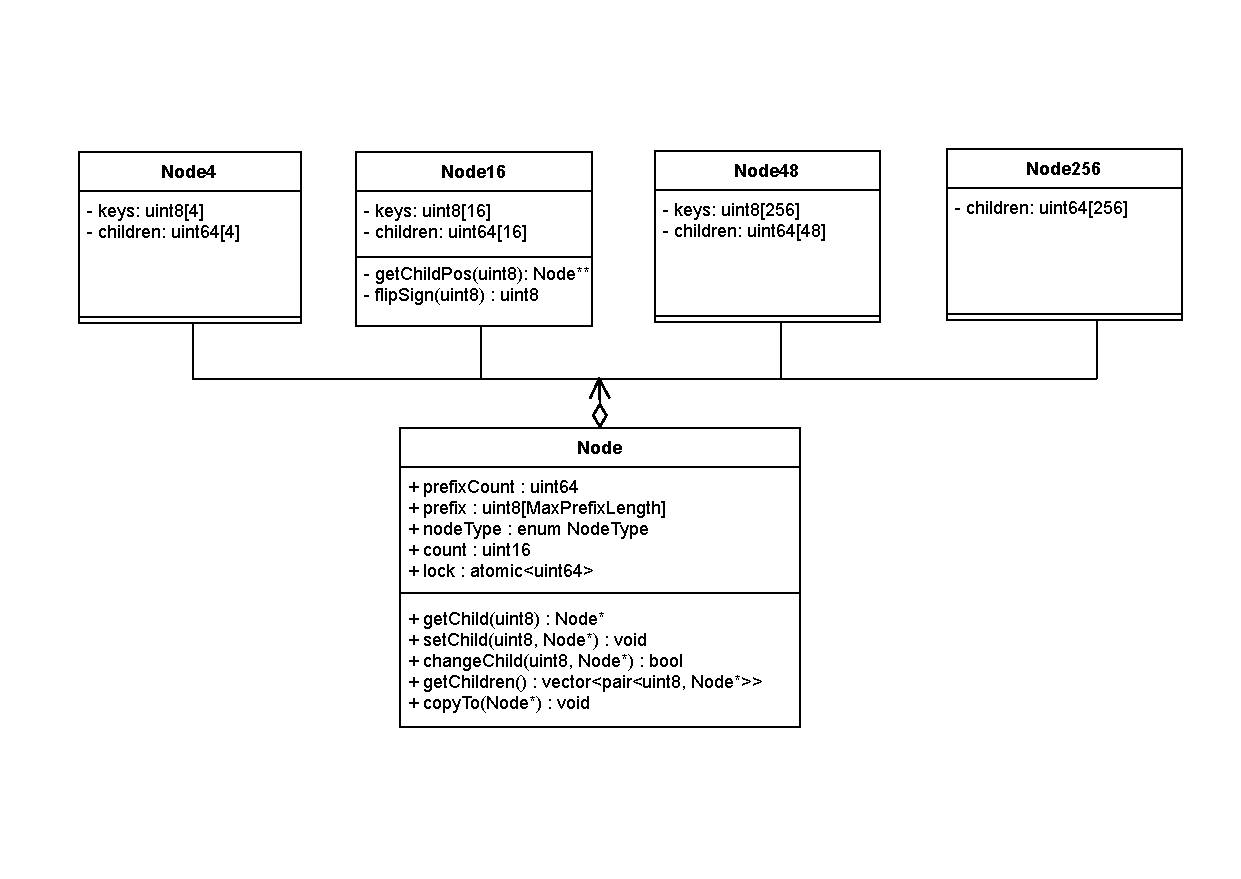
\includegraphics[width=1\textwidth]{ART-node-class.pdf}
  \caption{ART索引节点的类图}
  \label{fig:ART-node-class}
\end{figure}

\textbf{Node :}
\begin{itemize}
\item prefixCount : 公共前缀的长度,uint64类型

\item prefix[MaxPrefixLength] : 公共前缀,长度为MaxPrefixLength的字符串

\item nodeType : 节点的实际类型,enum {Node4, Node16, Node48, Node256} 类型

\item count : 节点中实际存储的子节点个数,uint16类型

\item lock : 前文中提到的乐观锁,std::atmoic<uint64>类型

\item getChild(): 返回key对应的孩子节点

\item setChild(): 设置某个孩子节点的指针,并将节点中子节点个数加1

\item changeChild(): 设置某个孩子节点的指针

\item getChildren(): 获得该节点的所有非空的孩子节点指针 
\end{itemize}

\textbf{Node4:}
\begin{itemize}
\item keys[4] : 子节点的键值,uint8类型数组

\item children[4] : 指向子节点的指针,uint64类型数组
\end{itemize}

\textbf{Node16:}
\begin{itemize}
\item keys[16] : 子节点的键值的补码,uint8类型数组

\item children[16] : 指向子节点的指针,uint64类型数组
\end{itemize}

\textbf{Node48:}
\begin{itemize}
\item keys[256] : keys[i]存储键值为i的子节点的在children数组中的索引,uint8类型数组

\item children[48] : 指向子节点的指针,为uint64类型数组
\end{itemize}

\textbf{Node256:}
\begin{itemize}
\item children[256] : 指向子节点的指针,uint64类型数组
\end{itemize}

以上为节点的私有的成员变量介绍,除此之外,节点还需要实现一些公共的方法,方便上层函数进行相关调用。这些接口包括getChild,setChild,changeChild,copyTo等。 
我们这里在基类中实现的是静态方法,在每种类型的子类节点都需要实现相应的方法。之后在父类中根据不同的
节点类型(前文中描述的NodeType)调用对应对象的方法。

针对不同的节点类型做的优化方法的实现:首先每一种类型的节点其内部的键值都是有序的,这一点是为了方便后续的范围查询。对于子节点数量最少的
Node4类型,按顺序查询相应的child即可,但是对于Node16类型,如果是循环查询对应的child,至多需要查询15次,效率明显下降,因此对于Node16类型的节点。
我们利用SIMD加速,一次操作128字节的keys。具体实现方法如下。

\begin{lstlisting} 
N *const *GetChildPos(const uint8_t k) const {
    __m128i cmp = _mm_cmpeq_epi8(_mm_set1_epi8(flipSign(k)),
        _mm_loadu_si128(reinterpret_cast<const __m128i *>(keys)));
    unsigned bitfield = _mm_movemask_epi8(cmp) & ((1 << count) - 1);
    if (bitfield) {
        return &children[ctz(bitfield)];
    } else {
        return nullptr;
    }
}

void SetChild(const uint8_t k, N *child) {
    uint8_t keyByteFlipped = flipSign(k);
    __m128i cmp = _mm_cmplt_epi8(_mm_set1_epi8(keyByteFlipped),
        _mm_loadu_si128(reinterpret_cast<__m128i *>(keys)));
    uint16_t bitfield = _mm_movemask_epi8(cmp) & (0xFFFF >> (16 - count));
    unsigned pos = bitfield ? ctz(bitfield) : count;
    memmove(keys + pos + 1, keys + pos, count - pos);
    memmove(children + pos + 1, children + pos, 
            (count - pos) * sizeof(N *));
    keys[pos] = keyByteFlipped;
    children[pos] = child;
    count++;
}
\end{lstlisting}

我们主要使用的是C++标准库中对SSE指令集的封装,\_mm\_cmplt\_epi8和\_mm\_cmpeq\_epi8分别支持对128bit的数据比较大小。前提是128bit其中存储的16个有符号数,
因此这里我们需要做一个转换flipSign(k)将传入的无符号k转换,便于使用有符号的SSE指令比较无符号数的大小。
\_mm\_cmplt\_epi8指的是两个128bit数每8bit比较大小,返回128bit的结果,其中每8bit为对应的两个8bit比较出的结果,返回1表示小于成立,否则返回0.
\_mm\_movemask\_epi8将结果转换为16bit的整型,ctz主要是计算实际的比较的结果中末尾存在0的个数。并根据此计算出应该将对应的k插入到具体的位置。

对于GetChildPos接口,主要是被getChild等查询子节点的函数调用,原理类似与上面setChild,但是SIMD指令稍有不同,这里是查询对应的k在索引节点中是否存在因此
选取的就是\_mm\_cmpeq\_epi8指令,比较的是对应的位置上是否有8bit的数据也就是key与目标key相同,若有相同返回1,没有相同则返回全0。
随后\_mm\_movemask\_epi8将结果转换为16bit的整型,再与((1 << count) - 1)相与,判断是否有k满足条件。

对于Node48,则是存储了256个key和48个槽位。每一个key中存储的都是对应槽位的索引,因此仅需要将无效的槽位标记为48。有效槽位的索引不可能大于48。
由此来降低在每个索引内部节点查询下层子节点的开销。

对于Node256,则是最基本的前缀树存储,只存储对应的256个指向子节点的指针,我们只需要通过的键值中对应位置的byte作为索引即可获得对应的子节点指针。
 
以上是在实现每一种Node节点类型时在工程上作出的优化,通过利用SIMD等操作,大大降低节点插入和查询的开销。对于Node48,通过在keys数组中
存储children数组索引的方式,用空间换取时间,也可以降低查询的开销。
\section{索引乐观锁实现}

上面提到的索引节点结构中,lock即为索引节点的乐观锁实现。以下为Node基类中关于lock的通用接口。

\begin{itemize}

\item ReadlockOrRestart(): 获得当前节点的读锁,若写标记或删除标记为1,则restart;否则返回当前的版本号

\item writeLockOrRestart(): 获得当前节点的写锁,若写标记或删除标记为1,则restart;否则版本增加1

\item upgradeLockOrRestart(): 将当前的读锁升级为写锁,若与读锁的版本号不一致,则restart;否则版本增加1

\item ReadUnlock(): 释放读锁,即比较当前版本号与先前版本号,若一致,返回成功;不一致,则restart

\item writeUnlock(): 释放写锁,即将当前节点的版本号加一

\item writeUnlockObsolete(): 释放写锁,并将节点标记为删除

\end{itemize}

以上对节点的锁的通用接口都被认为是具备原子性的。所有的对lock的修改操作都是通过c++中针对原子变量的操作
如lock.compare\_exchange\_strong()或者lock.fetch\_add()等。此外我们还需要设计使线程挂起的接口。
前文中提到当操作线程一直重启时,需要使线程挂起,等待系统冲突降低时,再执行该任务。
这里只需要使用系统中sched\_yield()调用,表示放弃当前的CPU即可。上面接口中的restart表示,当线程想要获得
锁被其他线程持有,或者是在获得锁到释放锁期间,有其他线程修改过锁时,该线程都会放弃这次操作,回到索引的
根节点重新开始一次操作。这在实现时可以使用一个goto语句实现。

\section{索引的并发控制机制}

\begin{figure}[h]
  \centering
  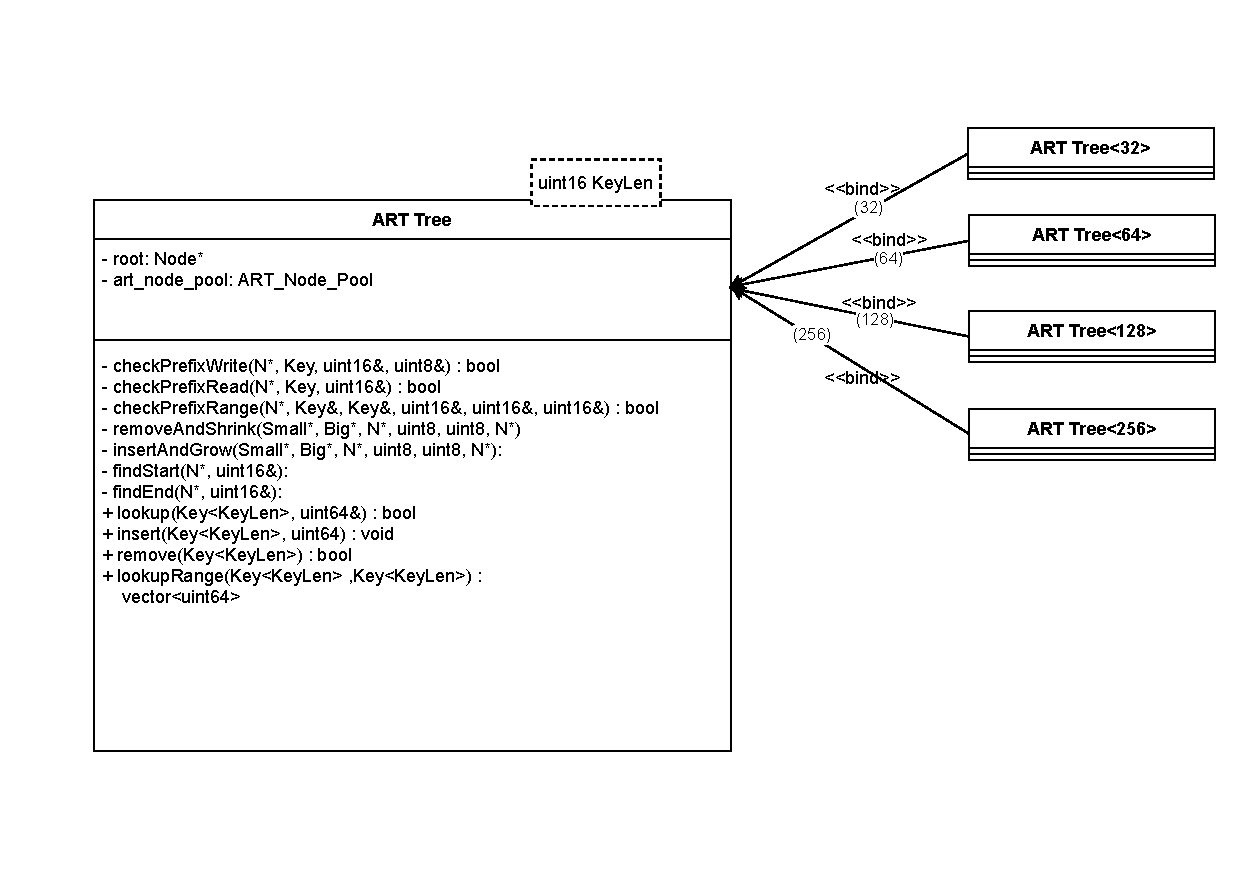
\includegraphics[width=1\textwidth]{ART-tree-class.pdf}
  \caption{ART Tree的类图}
  \label{fig:ART-tree-class}
\end{figure}

这一小节我们将介绍如何基于以上提到的数据结构和算法,实现ART索引的并发控制,对于ART来说主要需要实现以下几个public接口。
此外还需要实现针对内部结构的私有成员函数

\begin{itemize}

\item lookup(): 获得当前节点的读锁,若写标记或删除标记为1,则restart;否则返回当前的版本号

\item lookupRange(): 获得当前节点的写锁,若写标记或删除标记为1,则restart;否则版本增加1

\item insert(): 将当前的读锁升级为写锁,若与读锁的版本号不一致,则restart;否则版本增加1

\item delete(): 释放读锁,即比较当前版本号与先前版本号,若一致,返回成功;不一致,则restart

\end{itemize}

除了以上的公共的接口,索引还需要提供以下的私有函数,主要是为了解决节点伸缩问题以及处理不同类型操作中,
使用不同的前缀比较函数接口。


\begin{itemize}

\item removeAndShrink(): 删除对应的子节点的key和对应的孩子节点指针,并将当前节点缩容为更小的节点类型。
通过copyTo接口将剩下的keys和children拷贝到缩容后的新节点上。
同时修改父亲节点中对应的子节点指针,并将缩容前的节点做标记删除处理

\item insertAndGrow(): 申请节点容量更大的新节点,
通过copyTo接口将当前节点的keys和children拷贝到扩容后的新节点上。
插入对应的子节点的key和对应的孩子节点指针,
同时修改父亲节点中对应的子节点指针,并将扩容前的节点做标记删除处理

\item checkPrefixRead(): 对应查询/删除操作时的比较前缀的函数,当前缀不相等时,返回false,前缀相同的时候返回true

\item checkPrefixWrite(): 对应插入操作时的前缀比较函数,前缀不相等时返回false,同时也会返回不相等的key,以及相等部分的长度
前缀完全匹配时返回true

\item findStart(): 针对范围查询的辅助函数,差摘查找对应的上边界中是否有满足条件的结果,并返回结果集。

\item findEnd(): 针对范围查询的辅助函数,差摘查找对应的下边界中是否有满足条件的结果,并返回结果集。

\item checkPrefixRange(): 对应范围查询时,比较前缀与实际搜索的key的大小关系,若当前前缀在范围查询的[begin, end]之间
返回true,并且返回一个封闭区间[startKey, endKey],表示满足条件的区间查询的结果。针对上下边界可以使用上述的两个辅助函数进行
递归查询。最后合并 findStart(startKey), findEnd(endKey)以及(startKey, endKey)开区间上所有叶子节点。

\end{itemize}

以上分别介绍了索引实际操作的算法的接口下面我结合伪代码详细解释操作算法的实现过程。

\subsection{查询操作的实现}
对于ART索引来说,查询操作是一个最常用的操作,也是较为简单的一个操作,在查询操作中不涉及节点类型的变更,
也不涉及索引结构的修改。查询只需要从根节点开始,向下查询。每次进入当前节点时读取版本号,随后比较前缀,
若匹配进入下一层节点。在此之前,比较版本号是否存在变更。如此不断向下搜索直至找到对应的叶子节点。最后如果对应的
槽位上不含有指向子节点的指针,则返回Null。

\begin{breakablealgorithm} 
\counterwithin{algorithm}{chapter}
    \caption{ART索引查询流程伪代码} 
    \begin{algorithmic}[1]
    \begin{footnotesize}
    \hspace*{\algorithmicindent} \textbf{Input}{: key}\\
    \hspace*{\algorithmicindent} \textbf{Output}{: tid}
    \STATE {$cur \leftarrow root$}
    \STATE {$parent \leftarrow null$}
    \STATE {$level \leftarrow 1$}
    \WHILE{$level < KeyLen(key) $} 
        \STATE {$ReadLock(cur, v, needRestart)$}
        \STATE {$nextLevel \leftarrow level$}

        \IF{$checkPrefixRead(cur, key, level)$} 
            \STATE {$parent \leftarrow cur$}
            \STATE {$cur \leftarrow GetChild(cur, key[level])$}
            \STATE {$ReadCheck(parent, v, needRestart)$}

            \IF {$cur = null$} 
                \RETURN {false}
            \ENDIF

            \IF {$IsLeaf(cur) \And level = KeyLen(key)$}
                \STATE {$ReadUnlock(parent, v, needRestart)$}
                \STATE {$tid \leftarrow GetLeaf(cur)$}
                \RETURN {true}
            \ENDIF
        \ELSE 
            \STATE {$ReadUnlock(cur, v, needRestart)$}
            \RETURN {false}
        \ENDIF
        \STATE {$level \leftarrow level + 1$}
        \STATE {$ReadUnlock(cur, v, needRestart)$}
    \ENDWHILE
    \end{footnotesize}
    \end{algorithmic}
\end{breakablealgorithm}

\subsection{插入操作的实现}
索引的插入操作与查询操作最大的不同在于,前缀比较时,若不一致,则需要分裂当前节点,抽出最长的公共前缀。
此外,插入节点时可能会导致节点的扩容成容量更多的节点。整体的插入流程如下:从根节点开始,向下搜索,匹配
前缀,若不一致,申请新的Node4类型的节点,将公共前缀放入新申请的节点中,并且为新插入的key申请新的节点,
将curNode和nextNode插入newNode中,完成本次插入。若前缀一致,则需要查找对应的槽位是否有空缺,若不存在
子节点,则将nextNode插入对应的槽位,否则继续向下搜索,重复以上过程,直至节点可以被插入树中。

这里有个地方需要注意,实际我们编写代码时,没有使用路径压缩机制,实际如果我们使用路径压缩方式,不管是
查询还是插入,如果是采用路径压缩方式,则需要根据TID到数据库表中读取相应的字段,最后将各个字段组合成完整的
key,与需要比较的键值进行比较,这一步在内存数据库中,需要经过多次的访存,由于底层存储格式为行列混存。与一般
的行存不同,会导致读取多个字段的过程Cache是失效的。无法有效的利用CPU的Cache。而且,如果ART索引存储
的键值的长度都不会超长,每个节点的头节点部分存储着公共前缀。所以实际的树高是有限的,与多次访问
内存的开销相比也是可以忽略的。若树的节点都较为密集,而不是稀疏的存储一些值。那么压缩带来的优势也会大大降低。 
因此综上所述,我们并没有在实际实现时加入路径压缩,而是在路径上存储完整的键值。


\begin{breakablealgorithm} 
\counterwithin{algorithm}{chapter}
    \caption{ART索引插入流程伪代码} 
    \begin{algorithmic}[1]
    \begin{footnotesize}
    \hspace*{\algorithmicindent} \textbf{Input}{: key, tid}\\
    \hspace*{\algorithmicindent} \textbf{Output}{: void}
    \STATE {$cur \leftarrow null$} 
    \STATE {$next \leftarrow root$} 
    \STATE {$level \leftarrow 1$} 
    \WHILE{$level < KeyLen(key) $}
        \STATE {$parent \leftarrow cur$}
        \STATE {$cur \leftarrow next$}
        \STATE {$ReadLock(cur, v, needRestart)$}
        \STATE {$nextLevel \leftarrow level$}

        \IF{$!checkPrefixWrite(cur, key, nextLevel, noMatchKey, rePrefix, reLen)$} 
            \STATE // Prefix is not matched, split current Node
            \STATE {$CouplingLock(cur, parent, pv, v, needRestart)$}
            \STATE {$newNode \leftarrow new Node4()$}
            \STATE {$nextNode \leftarrow GenNewNode(key, nextLevel + 1, tid)$}
            \STATE {$newNode.SetPrefix(cur.GetPrefix(), nextLevel - level)$}
            \STATE {$cur.SetPrefix(remainPrefix, remainLen)$}

            \STATE {$SetChild(newNode, noMatchKey, cur)$}
            \STATE {$SetChild(newNode, key[nextLevel], nextNode)$}
            \STATE {$ChangeChild(parent, pk, newNode)$}

            \STATE {$WriteUnlock(cur)$}
            \STATE {$WriteUnlock(parent)$} 
        \ENDIF
        \STATE {$k \leftarrow key[nextLevel]$}
        \IF{$!GetChild(cur, k)$} 
            \STATE // current child pointer is null
            \IF{$cur.IsFull()$}
                \STATE // current node is full, should grow to bigger one.
                \STATE {$CouplingLock(cur, parent, pv, v, needRestart)$}
                \STATE {$InsertAndGrow(cur, parent, pk, k, GenNewNode(key, nextLevel + 1, tid))$}
                \STATE {$DeleteUnlock(cur)$}
                \STATE {$WriteUnlock(parent)$}
                \STATE {$markNodeForDeletion(cur)$}
            \ELSE 
                \STATE // current node is not full, insert tid into current node.
                \STATE {$UpgradeLock(cur, v, needRestart)$}
                \STATE {$SetChild(cur, k, GenNewNode(key, nextLevel + 1, tid))$}
                \STATE {$WriteUnlock(cur)$}
            \RETURN {}
            \ENDIF
        \ELSE
            \STATE {$next \leftarrow GetChild(cur, k)$}

            \IF{$IsLeaf(next)$}
                \STATE // The same Key is thought as update
                \STATE {$UpgradeLock(cur, v, needRestart)$}
                \STATE {$ChangeChild(cur, k, tid)$}
                \STATE {$WriteUnlock(cur)$}
                \RETURN {}
            \ENDIF

            \IF{$parent != null$} 
                \STATE {$ReadUnlock(parent, pv, needRestart)$}
            \ENDIF
        \ENDIF
        
        \STATE {$level \leftarrow nextLevel + 1$}
    \ENDWHILE
    \end{footnotesize}
    \end{algorithmic}
\end{breakablealgorithm}

\subsection{删除流程操作}
索引的删除操作可以理解为特殊的插入操作,在进行前缀比较时,与查询操作比较类似,只有前缀匹配和不匹配的情况。
当前缀不匹配时说明此时索引中不存在需要被删除的记录,因此函数直接返回即可。若前缀匹配则继续查询。
当对应的槽位上为叶子节点时,则可以执行删除操作。删除操作需要注意的是可能会引起节点收缩,因此需要申请更小类型的
节点,将剩余的键值和对应的孩子节点指针拷贝到新的节点中哦,同时还需要将原节点标记删除。最后需要将父亲节点中的子节点指针修改
为新申请节点的地址。


\begin{breakablealgorithm} 
\counterwithin{algorithm}{chapter}
    \caption{ART索引删除流程伪代码} 
    \begin{algorithmic}[1]
    \begin{footnotesize}
    \hspace*{\algorithmicindent} \textbf{Input}{: key}\\
    \hspace*{\algorithmicindent} \textbf{Output}{: void}
    \STATE {$cur \leftarrow null$} 
    \STATE {$next \leftarrow root$} 
    \STATE {$level \leftarrow 1$} 
    \WHILE{$level < KeyLen(key) $}
        \STATE {$parent \leftarrow cur$}
        \STATE {$cur \leftarrow next$}
        \STATE {$ReadLock(cur, v, needRestart)$}
        \STATE {$nextLevel \leftarrow level$}

        \IF{$!checkPrefixWrite(cur, key, nextLevel, noMatchKey, rePrefix, reLen)$} 
            \STATE // Prefix is not matched, split current Node
            \STATE {$CouplingLock(cur, parent, pv, v, needRestart)$}
            \STATE {$newNode \leftarrow new Node4()$}
            \STATE {$nextNode \leftarrow GenNewNode(key, nextLevel + 1, tid)$}
            \STATE {$newNode.SetPrefix(cur.GetPrefix(), nextLevel - level)$}
            \STATE {$cur.SetPrefix(remainPrefix, remainLen)$}

            \STATE {$SetChild(newNode, noMatchKey, cur)$}
            \STATE {$SetChild(newNode, key[nextLevel], nextNode)$}
            \STATE {$ChangeChild(parent, pk, newNode)$}

            \STATE {$WriteUnlock(cur)$}
            \STATE {$WriteUnlock(parent)$} 
        \ENDIF
        \STATE {$k \leftarrow key[nextLevel]$}
        \IF{$!GetChild(cur, k)$} 
            \STATE // current child pointer is null
            \IF{$cur.IsFull()$}
                \STATE // current node is full, should grow to bigger one.
                \STATE {$CouplingLock(cur, parent, pv, v, needRestart)$}
                \STATE {$InsertAndGrow(cur, parent, pk, k, GenNewNode(key, nextLevel + 1, tid))$}
                \STATE {$DeleteUnlock(cur)$}
                \STATE {$WriteUnlock(parent)$}
                \STATE {$markNodeForDeletion(cur)$}
            \ELSE 
                \STATE // current node is not full, insert tid into current node.
                \STATE {$UpgradeLock(cur, v, needRestart)$}
                \STATE {$SetChild(cur, k, GenNewNode(key, nextLevel + 1, tid))$}
                \STATE {$WriteUnlock(cur)$}
            \RETURN {}
            \ENDIF
        \ELSE
            \STATE {$next \leftarrow GetChild(cur, k)$}

            \IF{$IsLeaf(next)$}
                \STATE // The same Key is thought as update
                \STATE {$UpgradeLock(cur, v, needRestart)$}
                \STATE {$ChangeChild(cur, k, tid)$}
                \STATE {$WriteUnlock(cur)$}
                \RETURN {}
            \ENDIF

            \IF{$parent != null$} 
                \STATE {$ReadUnlock(parent, pv, needRestart)$}
            \ENDIF
        \ENDIF
        
        \STATE {$level \leftarrow nextLevel + 1$}
    \ENDWHILE
    \end{footnotesize}
    \end{algorithmic}
\end{breakablealgorithm}

\subsection{范围查询流程}
范围查询是索引中较为常用的操作,比如 select * from t1 where t1.a < 100 and t1.a > 10, 如果在t1.a上建立了
索引那么该查询就会使用索引的范围查询,读取出存储数据的TID的集合,在根据这个集合回表读取实际需要的数据。

(以下讨论中key代表需要查询的key值,类型为Key<KeyLen>, k代表key中的一个字节,类型为byte。)
范围查询的详细流程设计如下,从根节点开始向下读取。针对每一个节点,首先检查当前节点的前缀,如果完全该前缀不在查询的区间内,返回false。
若该前缀在闭区间[key1, key2]之间,通过copy函数返回该节点上所有叶子节点的并集。
若该前缀与闭区间[key1, key2]对应的前缀相等,则查询当前节点上的满足区间[key1[level], key2[level]]的孩子节点指针。
这里需要注意开闭区间的问题,由于存储的数据是离散的,而查询的范围是连续的,对于恰好满足node.keys[pos] = key1[level]
的子节点指针。还需要递归向下继续查询。同理对于满足node.keys[pos] = key2[level]的子节点,也需要继续向下搜索满足条件的
结果。这里我们使用两个Lambda表达式findStart和findEnd。最后我们将开区间 (key1[level], key2[level]) 上的所有
叶子节点和通过findStart和findEnd查询出的结果集做并集,返回查询结果。查询过程中,整个都是通过读锁的方式进行并发控制,流程
参考单点查询过程。详细的实现见下图中的伪代码。

\begin{breakablealgorithm} 
\counterwithin{algorithm}{chapter}
    \caption{ART索引范围查询流程伪代码} 
    \begin{algorithmic}[1]
    \begin{footnotesize}
    \hspace*{\algorithmicindent} \textbf{Input}{: k1, k2}\\
    \hspace*{\algorithmicindent} \textbf{Output}{: tids}
    \STATE {$cur \leftarrow root$}
    \STATE {$parent \leftarrow null$}
    \STATE {$level \leftarrow 1$}
    \WHILE{$level < KeyLen(key) $} 
        \STATE {$ReadLock(cur, v, needRestart)$}
        \STATE {$nextLevel \leftarrow level$}

        \IF{$checkPrefixRead(cur, k1, k2, level, startkey, endkey)$} 
            \STATE {$children \leftarrow GetChildren(cur, startkey, endkey)$}

            \IF {$len(children) >= 2$} 
                \FOR {$child in children$}
                    \IF {$child = k1[level]$}
                        \STATE {$findStart(child)$}
                    \ELSIF {$child = k2[level]$}
                        \STATE {$findEnd(child)$}
                    \ELSE
                        \STATE {$copy(child)$}
                    \ENDIF    
                \ENDFOR
            \ELSIF {$len(children) = 1$} 
                \STATE {$cur \leftarrow GetChild(cur, k1[level])$}
            \ENDIF
                \RETURN {false}
        \ELSE 
            \RETURN {false}
        \ENDIF
        \STATE {$level \leftarrow level + 1$}
        \STATE {$ReadUnlock(cur, v, needRestart)$}
    \ENDWHILE
    \end{footnotesize}
    \end{algorithmic}
\end{breakablealgorithm}

\begin{breakablealgorithm} 
\counterwithin{algorithm}{chapter}
    \caption{ART索引范围查询流程伪代码} 
    \begin{algorithmic}[1]
    \begin{footnotesize}
    \hspace*{\algorithmicindent} \textbf{Input}{: k1, k2}\\
    \hspace*{\algorithmicindent} \textbf{Output}{: tids}
    \STATE {$cur \leftarrow root$}
    \STATE {$parent \leftarrow null$}
    \STATE {$level \leftarrow 1$}
    \WHILE{$level < KeyLen(key) $} 
        \STATE {$ReadLock(cur, v, needRestart)$}
        \STATE {$nextLevel \leftarrow level$}

        \IF{$checkPrefixRead(cur, k1, k2, level, startkey, endkey)$} 
            \STATE {$children \leftarrow GetChildren(cur, startkey, endkey)$}

            \IF {$len(children) >= 2$} 
                \FOR {$child in children$}
                    \IF {$child = k1[level]$}
                        \STATE {$findStart(child)$}
                    \ELSIF {$child = k2[level]$}
                        \STATE {$findEnd(child)$}
                    \ELSE
                        \STATE {$copy(child)$}
                    \ENDIF    
                \ENDFOR
            \ELSIF {$len(children) = 1$} 
                \STATE {$cur \leftarrow GetChild(cur, k1[level])$}
            \ENDIF
                \RETURN {false}
        \ELSE 
            \RETURN {false}
        \ENDIF
        \STATE {$level \leftarrow level + 1$}
        \STATE {$ReadUnlock(cur, v, needRestart)$}
    \ENDWHILE
    \end{footnotesize}
    \end{algorithmic}
\end{breakablealgorithm}

\begin{breakablealgorithm} 
\counterwithin{algorithm}{chapter}
    \caption{ART索引范围查询流程copy伪代码} 
    \begin{algorithmic}[1]
    \begin{footnotesize}
    \hspace*{\algorithmicindent} \textbf{Input}{: k1, k2}\\
    \hspace*{\algorithmicindent} \textbf{Output}{: tids}
    \IF{$isLeaf(node)$}
            \STATE {$add node into result$}
    \ELSE
        \STATE {$children \leftarrow GetChildren(node, 0, 255)$}   
        \FOR {$child in children$}
            \STATE {$copy(child)$}
        \ENDFOR
    \ENDIF 
    \end{footnotesize}
    \end{algorithmic}
\end{breakablealgorithm}


\begin{breakablealgorithm} 
\counterwithin{algorithm}{chapter}
    \caption{ART范围查询中findStart伪代码描述} 
    \begin{algorithmic}[1]
    \begin{footnotesize}
   
    \STATE {$res = CheckPrefix(cur, level)$}
    \IF {$res > 0$}
        \RETURN
    \ELSIF {$res < 0$}
        \STATE {$copy(node)$}
    \ELSE
        \STATE {$children \leftarrow GetChildren(node, level, 255)$}
        \FOR {$child in children$}
            \IF {$child is first child$}
                \STATE {$findStart(child)$}
            \ELSE
                \STATE {$copy(child)$}
            \ENDIF 
        \ENDFOR
    \ENDIF  
    \end{footnotesize}
    \end{algorithmic}
\end{breakablealgorithm}

\begin{breakablealgorithm} 
\counterwithin{algorithm}{chapter}
    \caption{ART范围查询中findEnd的伪代码描述} 
    \begin{algorithmic}[1]
    \begin{footnotesize}
    \STATE {$res = CheckPrefix(cur, level)$}
    \IF {$res > 0$}
        \RETURN
    \ELSIF {$res < 0$}
        \STATE {$copy(node)$}
    \ELSE
        \STATE {$children \leftarrow GetChildren(node, 0, level)$}
        \FOR {$child in children$}
            \IF {$child is end child$}
                \STATE {$findEnd(child)$}
            \ELSE
                \STATE {$copy(child)$}
            \ENDIF 
        \ENDFOR
    \ENDIF  
    \end{footnotesize}
    \end{algorithmic}
\end{breakablealgorithm}

\section{内存管理模块的实现}
前面我们介绍了索引节点随着插入删除元素,节点类型的变更。节点类型变更需要将原来节点中数据拷贝到新的节点中,并对
原始节点做标记删除。但是我们并不能将该节点的内存立即归还操作系统。下图就是我们设计的基于无锁队列的内存管理。
所有被标记删除的节点都会被插入队列头部,由于索引在插入删除过程中经常性需要申请新的节点也是优先从该无锁队列获取,
若获取失败才会向系统申请。

根据前文所提到的两种管理内存的方式,下面我们来详细阐述是如何实现这两种内存管理机制。

\begin{figure}[h]
  \centering
  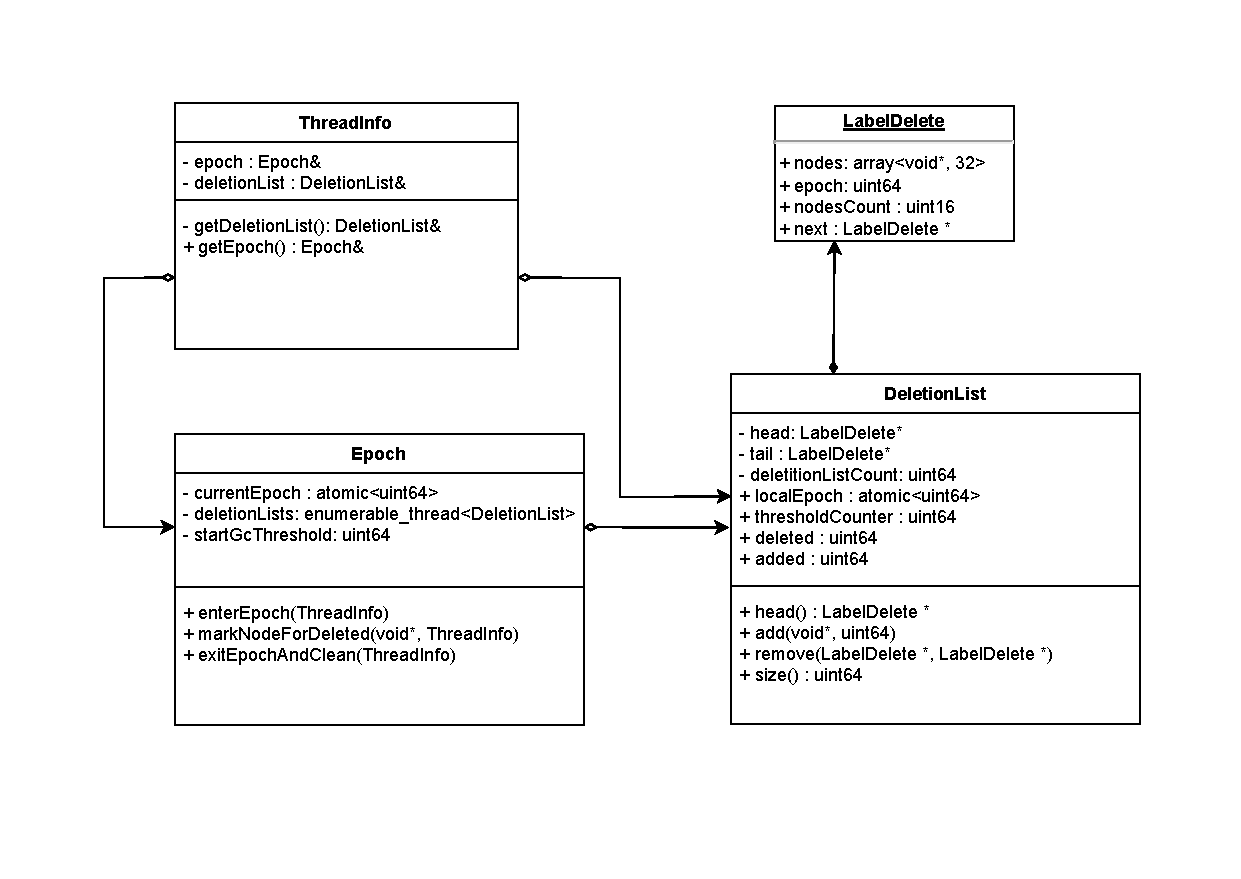
\includegraphics[width=1\textwidth]{art-epoch-gc.pdf}
  \caption{去中心化的垃圾回收类的类图}
  \label{fig:art-epoch-gc}
\end{figure}


两种内存管理机制分别是基于epoch的垃圾回收机制和基于无锁链表的垃圾回收机制。下图为基于epoch的垃圾回收的对象实现。
下面我们主要实现的是threadInfo类,epoch类。

对于epoch类,每个epoch会维护thread\_local的deleteList(被删除节点的链表),当前的epoch的信息以及一个垃圾删除的阈值
(低于该阈值的epoch上的标记删除节点可以真正的被回收),而threadInfo主要包含两个属性,分别是对epoch的引用和对待删除节点
列表的引用。

正常的流程如下,当某个工作线程T1需要对索引操作时,会根据当前索引中的epoch生成一个threadInfo .这里我们参考标准库中对mutex
的lock\_guard封装。采用RAII的思想,设计两个类EpocheGuard和EpocheGuardReadOnly
分别代表只读操作和读写操作需要对epoch和deletionList进行的操作,从而在使用上避免了直接对锁进行操作,减少了人为的死锁可能性。

对于epoch类,主要其三个主要的接口分别为enterEpoche(), markNodeForDeletion(), exitEpocheAndCleanup()

\begin{itemize}

\item enterEpoche(): 进入epoch,读取当前的epoch值

\item markNodeForDeletion(): 将节点标记删除,注册到deletionList中,待删除。这里的deletionList是threadLocal的,所以可以做到
线程间互不影响。

\item exitEpocheAndCleanup(): 退出当前的epoch,并根据此时需要删除的节点个数是否满足阈值要求,若达到要求则将其删除。
此处会遍历所有的deletionList,用到了intel提供的支持threadLocal的函数库,可以方便便利所有的threadlocal对象。

\end{itemize}

以上三个接口就可以完成去中心化的垃圾收集机制,由于需要依赖特定的函数库,因此可能在其他平台上并不适用,目前在x86平台上,这套
方案是比较稳妥且方便的。而且不会造成系统性能瓶颈。

对于不能够使用以上基于去中心化的垃圾回收机制的平台,此处还有一套基于无锁链表的垃圾回收机制。主要实现原理如下。
在索引模块中维护一个art\_obj\_pool对象,每次申请新的节点时都会向此对象申请内存,而如果需要删除某个节点,只需要将
删除的节点通过CAS插入链表的头部即可。

\begin{figure}[h]
  \centering
  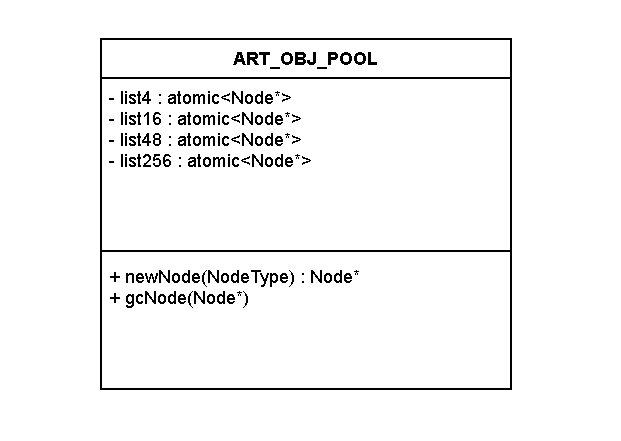
\includegraphics[width=0.9\textwidth]{art-obj-pool-class.pdf}
  \caption{无锁链表的垃圾回收类的类图}
  \label{fig:art-obj-pool-class}
\end{figure}

此方案有较大的改进空间,比如可以使用linux内核中常见的buddy内存分配算法,将小块的内存组合成大块,或者将大块的内存切分为
小块。
主要实现如下所示,当需要申请新的索引节点时,art\_obj\_pool会优先使用垃圾回收队列中的内存,根据申请的node类型,返回相应的
内存块,并在此基础上做初始化(placement new)。
这里有一点需要注意的是,对节点版本号应该继续加1,因为这里需要防止,节点刚刚被标记删除,随后就被回收,此时其他线程申请内存,
内存池返回该内存块,但是先前仍有其他内存持有该节点,此时,先前的线程认为节点可用,继续操作。因此我们在获得新的内存块时仍需要对其
版本号继续自增,这样先前的线程t2读取版本号发现已经变更,便会返回从根节点开始继续操作,而不会产生两个线程互相持有节点,导致节点操作异常。


\section{内存数据库表的组织方式}
结合以上的阐述,内存数据库中表的组织方式,目前数据库的表主要是以PAX方式进行组织。以4Mb为最基本的存储单位,每个block需要
做到4Mb字节的对齐。内存数据库中所有数据均存储在内存中,因此索引中的value只需要存储相应的记录的实际地址。针对PAX行列混存。
每个block内部的数据组织如下图。

\begin{figure}[h]
  \centering
  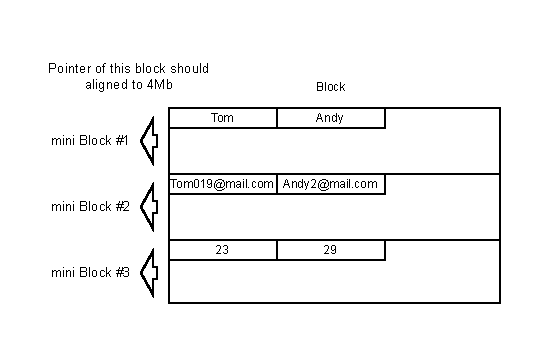
\includegraphics[width=0.9\textwidth]{PAX-class.pdf}
  \caption{PAX存储的内存布局}
  \label{fig:PAX-class}
\end{figure}

每个block内部数据按照列式存储,首先存储的是关于block的基本信息,其后为了实现上层事务中的MVCC事务并发控制。第一列存储对应
每一行的版本号指针,指向的是每一条undo log,实现多版本并发控制。其后存储的才是真正的数据。由于实际存储中可能会存在变长字段的
问题,解决这个问题可以引入一个全局的或者表级的变长字段管理器,所有变长字段可以作为一个长度为16字节的字段,如果长度小于8字节,
则直接存储在对应的block中,若长度大于8字节,则block中存储长度和地址,根据这两个参数到变长字段管理器,查询或者修改该字段的值。

索引中每一个叶子节点指向的都是版本号指针的地址,应用block头部的基本元信息,可以获取完整的一条记录。下图为block对外暴露的接口。
主要用于对表的修改,点查询,范围查询。

\begin{figure}[h]
  \centering
  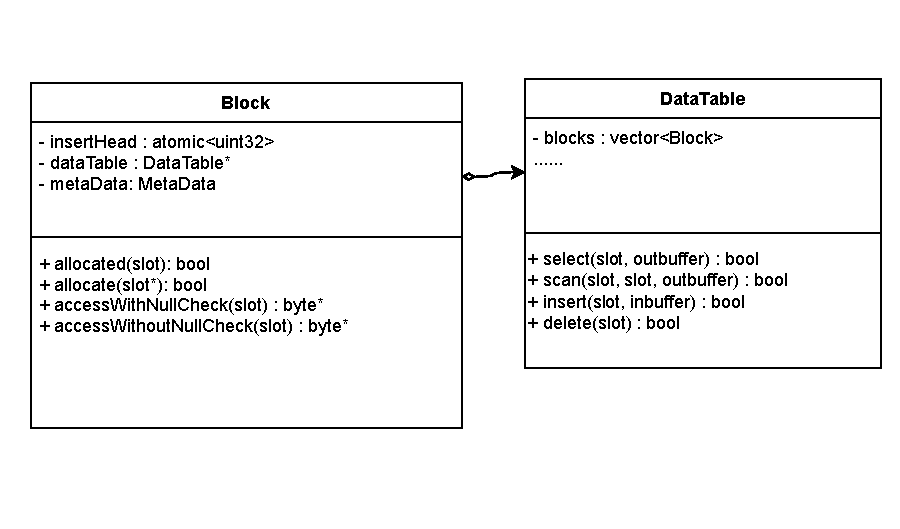
\includegraphics[width=0.9\textwidth]{PAX-class-2.pdf}
  \caption{PAX存储底层实现类的类图}
  \label{fig:PAX-class-2}
\end{figure}

\section{数据库索引的创建与管理的实现}

上述章节中详细介绍了数据库索引的结构,操作算法,内存管理,索引与表的联系,索引与事物的联系。作为本章的最后一个小节
将讨论索引最常规的操作就是create index 和drop index。本数据库中这两个操作都作为一个事务行操作,即允许其与其他DML操作
并发进行,而不会造成数据库一致性问题。

结合上文中提到的DAF模块,drop index的操作作为一个deferred action被注册到DAF Manager中。在这个deferred action中仍是一个
lambda表达式,表示这个动作还会被延迟执行。如下图所示。当前DAF Manager中有 drop index以及 对索引的插入操作。当daf执行
drop index时,会注册一个新的延迟操作到DAFmanager中,因此后面执行的对索引的插入操作仍然是可以进行的,不会造成插入一个空的
索引的问题。

而对于索引的生成则没有上述问题。索引创建主要是根据实际需要索引的字段创建相关的索引。根据之前章节所述的各种数据类型和索引key之间的
转换规则,如下,将实际的数据类型转换为索引中的key。作为keySchema传入indexBuilder,indexBuilder根据需要生成索引类型。
创建相关数据结构。并修改数据库系统中元数据。

以上是针对索引的创建和删除操作的实现,由于事务部分不是本片文章的重点,因此这里只是简单介绍一下关于如何处理索引的创建和删除过程
以下是一个完整的实现图。


\section{本章小结}

本章内容主要是从软件工程的角度,分析阐述如何实现具体的ART索引,以及基于乐观级联锁的方式处理对索引结构的并发操作。
分析了索引结构内存管理相关内容,以及如何将不同类型的数据组合成可以存储在索引中的键值数据。最后介绍了关于索引的DDL相关的
操作,简单描述DAF事务处理框架可以处理索引创建删除等操作,而不会引起任何内存或者其他一致性问题。 % art 索引详细设计
% !TeX root = ../main.tex

\chapter{实验测试和分析}

基于上述章节,本章将对实现的ART索引进行相关的功能性测试和性能测试。
并且分析在有垃圾回收和无垃圾回收时内存使用情况。

\section{测试环境}

\subsection{硬件测试环境}
本次测试主要由一台主机完成,如下表所示其配置如下

% \usepackage{caption}

\begin{table}
\centering
\captionsetup{labelformat=empty}
\caption{服务器配置}
\begin{tabular}{|l|l|} 
\hline
cpu                  & ecs.c7a.8xlarge 32 vCPU       \\ 
\hline
内存                   & 64G      \\ 
\hline
硬盘                   & ESSD云盘 256GB  \\ 
\hline
操作系统                 & Ubuntu 20.04 (5.04.4)    \\ 
\hline
\multicolumn{1}{l}{} & \multicolumn{1}{l}{}    
\end{tabular}
\end{table}

\subsection{测试数据集和框架}
本次测试针对功能性测试主要测试索引插入,查询,范围查询,删除操作这些功能是否正确。
采取多种不同类型的数据(包括Int, Double,String)进行相关测试。除此之外,选取数据集时分别有顺序集合和随机集合。
依赖Google的GTest测试框架进行全面的测试。

\section{功能性测试}

针对功能性测试,主要测试索引操作算法的正确性,包括单线程,多线程操作的正确性,支持最长匹配的索引查询的正确性。

因此我们这里针对普通索引,使用Ints类型数据集和String类型数据集。根据插入顺序,生成1000万条数据。为了保证测试的
覆盖率。除了递增的数据之外,还需要对插入,查找随机数据集合。

\section{性能测试}
上述小节主要测试索引的功能性测试。本小节主要设计针对索引的性能测试。主要对比的是应用乐观级联锁之后,索引操作的可扩展
性是否达到预期要求。下面所有测试都是针对的并发读写的场景,考虑单一类型操作和读写混合操作。

\subsection{查询性能测试}

\begin{figure}[h]
  \centering
  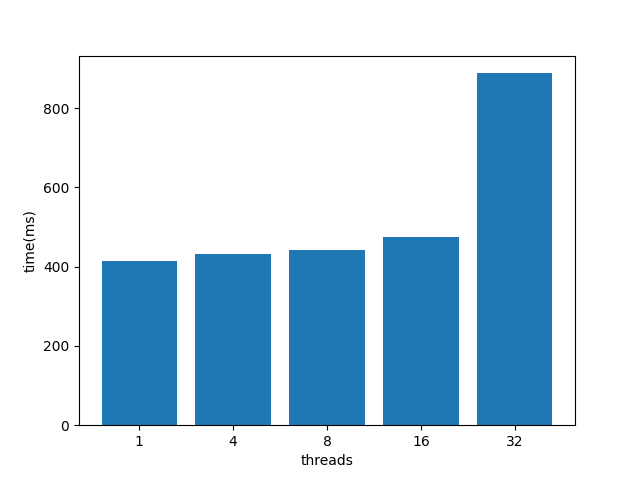
\includegraphics[width=0.9\textwidth]{lookup1.png}
  \caption{并发查询1000万条有序记录时间}
  \label{fig:cc-lookup-1}
\end{figure}

\begin{figure}[H]
  \centering
  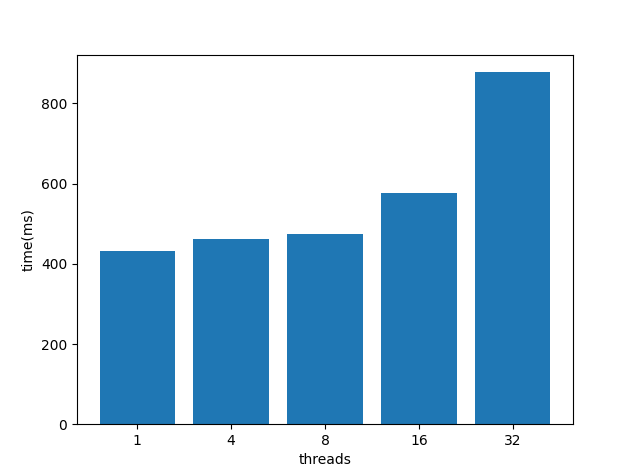
\includegraphics[width=0.9\textwidth]{lookup2.png}
  \caption{并发查询1000万条随机记录时间}
  \label{fig:cc-lookup-2}
\end{figure}

对于查询的性能测试,主要设计的数据集为1000万条,首先系统导入这1000万条数据,随后分别由1,4,8,16,32个线程进行查询测试
测试的结果如上图所示,以下表中包括顺序查询,随机点查询。

针对顺序数据的查询,1至16个工作线程分别查询1000万记录的耗时基本相同,但是32线程查询时,由于测试平台的核数仅有32个vCPU,这里导致线程调度的开销切换过大,
导致影响了正常的索引查询操作。造成一个突出的峰值。

针对随机数据的查询,综合上图的结果来看,与顺序查询的结果基本一致,即是乐观锁对于只读操作来说,多核扩展性较为友好。

\subsection{插入性能测试}

\begin{figure}[H]
  \centering
  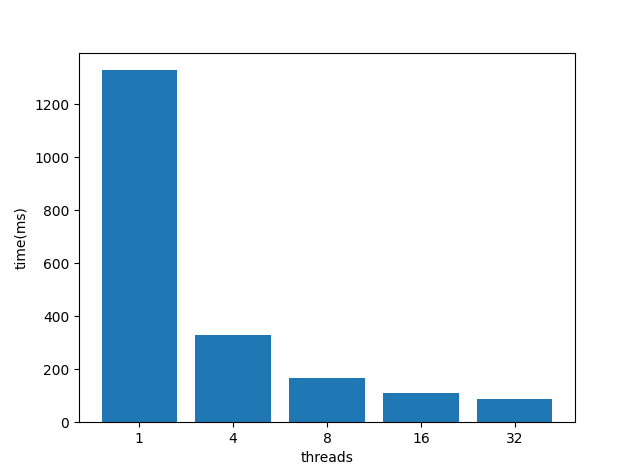
\includegraphics[width=0.9\textwidth]{insert1.png}
  \caption{并发插入1000万条有序记录时间}
  \label{fig:cc-insert-1}
\end{figure}

\begin{figure}[H]
  \centering
  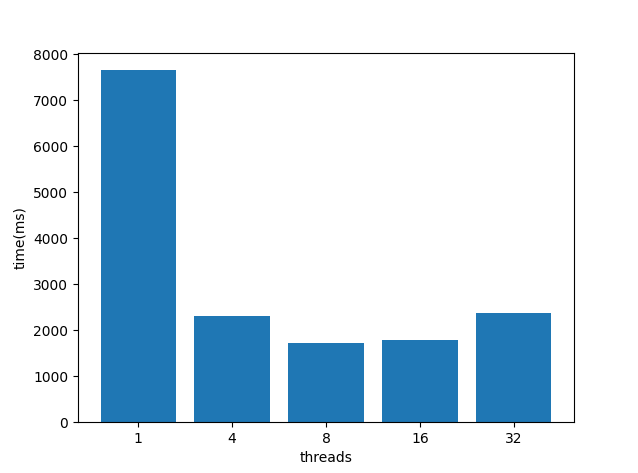
\includegraphics[width=0.9\textwidth]{insert2.png}
  \caption{并发插入1000万条随机记录时间}
  \label{fig:cc-insert-2}
\end{figure}


针对插入的性能测试,主要设计的数据集为1000万条,分别由1,4,8,16,32个线程进行插入测试,所有测试的总的数据记录的个数是相同的。即是最后
当所有线程操作完成之后,ART索引中都是只包含1000万条记录。
测试的结果如上图所示。

需要注意的是以下的插入数据分为两种。前者线程间插入的键值是互相离散的,即每个线程只负责插入某个区间的值,且区间和区间之间是完全不
重叠的,此时冲突较小。而后者我们可以看到同样是插入1000万条记录,对比同样的线程数,随机插入的吞吐量只有前者的十分之一。
这是因为当线程间插入随机数据时可能会频繁争用同一个索引内部节点时,导致冲突较大,在我么的索引实现中,采取的是当冲突增多之后的避让机制,这必然会导致线程挂起和睡眠。
因此多线程并行插入的效率就会产生较大的问题。

由此可以说明乐观锁的方式并不适合写冲突较高的场景,因为当写冲突较多操作会不断回到根节点,然后执行重做。如果当前的操作的深度
过大,则执行重做的开销较大,会造成系统性能抖动,因此乐观锁的并发控制确实不适合写冲突高的场景。

\subsection{删除性能测试}

删除的性能测试和以上插入测试类似,当删除操作需要删除的数据记录之间重叠较多,并行删除的效率会大大降低。由此得出的结论与并发插入
时是一致的。就是基于乐观锁的ART索引并不适合作为需要被频繁修改的索引结构。

\begin{figure}[H]
  \centering
  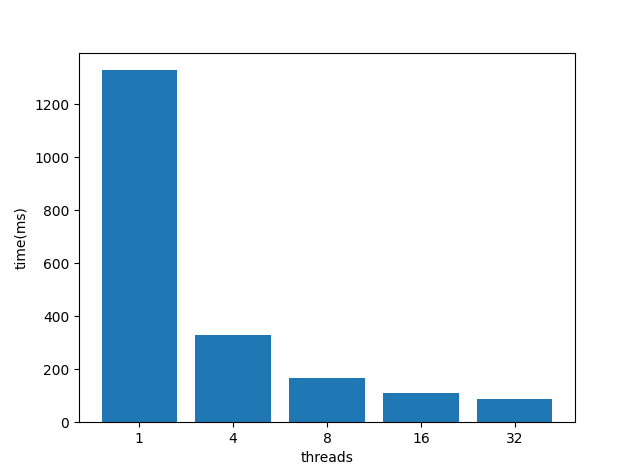
\includegraphics[width=0.9\textwidth]{delete1.png}
  \caption{并发删除1000万条有序记录时间}
  \label{fig:cc-delete-1}
\end{figure}

\begin{figure}[H]
  \centering
  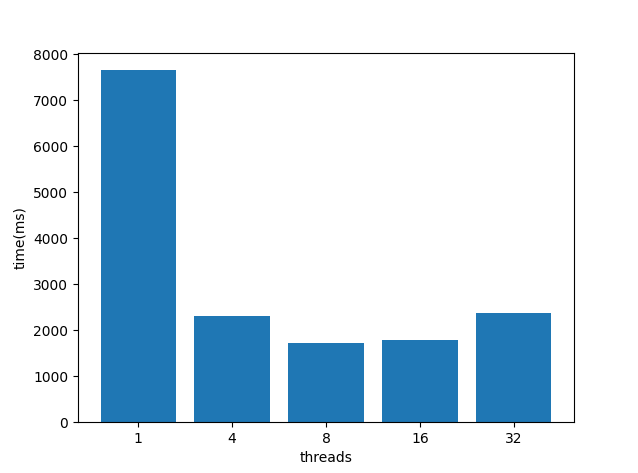
\includegraphics[width=0.9\textwidth]{delete2.png}
  \caption{并发删除1000万条随机记录时间}
  \label{fig:cc-delete-2}
\end{figure}

这里删除的性能测试结果与插入较为类似,也是一开始随着工作线程增多而获得较大的性能提升,但是随着工作线程的继续增加,所获得的
提升越小,甚至产生了副作用。

\subsection{查询/插入性能测试}

上述的测试中,只是针对单一的类型的负载进行测试,但是在实际应用中,并不存在只读或者只写类型的负载。
因此我们还设计了读写并行的测试数据。

\begin{figure}[H]
  \centering
  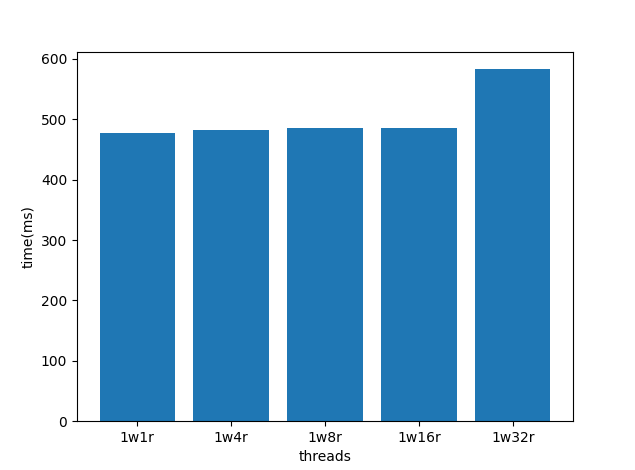
\includegraphics[width=0.9\textwidth]{rw.png}
  \caption{一写多读负载下的总耗时}
  \label{fig:rw}
\end{figure}

对于查询和插入的并行测试,主要是测试实际使用场景下多读单写情况,如下图所示,工作线程分为读线程和写线程,
分别为1写1读,1写4读,1写8读,1写16读,1写32读。测试其在并发情况下的性能,图中表明,随着并发线程的个数增长,完成所有操作需要的
时间并没有明显上升。表明基于乐观级联锁的ART索引在多核多线程使用场景下具备扩展性,基本满足设计预期。


\section{内存开销测试}

\begin{figure}[H]
  \centering
  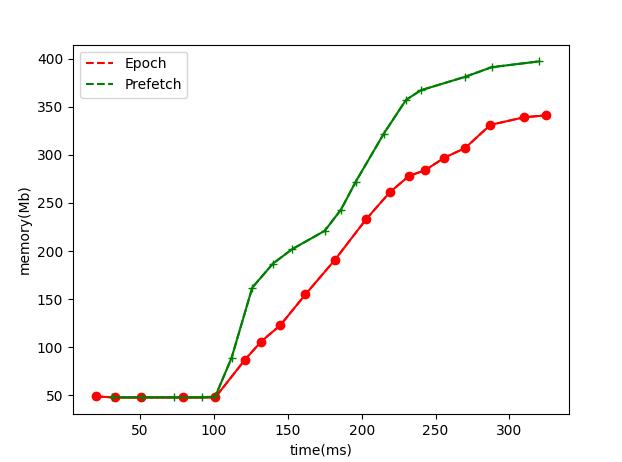
\includegraphics[width=0.9\textwidth]{memory.png}
  \caption{内存开销统计}
  \label{fig:memory}
\end{figure}


内存开销测试主要是针对不同数据量下,内存使用的开销,主要测试目的除了实际内存占用外,还需要测试在基于epoche的垃圾回收机制
对索引性能的影响。最终我们在多个数据量下进行测试,分别对比开启垃圾回收和不开启垃圾回收的吞吐量和内存开销。根据下图所示,在小数据量下
使用基于epoch的垃圾回收的效果较使用无锁队列收集删除节点差,但是在大数据量下,尤其是接近系统的上限时,由于此时操作系统内存较多
导致此时索引速度明显降低。因此我们在索引中设置一个阈值,超过阈值才会启动基于epoch的垃圾回收机制。这样两者结合可以获得较大的性能提升。

\section{本章小结}

本章主要介绍前文中设计和实现的基于乐观级联锁的索引及其相关模块的测试,第一小节介绍实际测试的环境,第二节针对前文中提到的相关
功能进行功能测试,第三节中主要进行相关性能测试,主要测试目的在于测试该索引在性能上是否达到所预期的效果,尤其是在多读少写的场景下
是否达到预期的效果。综合上述的测试也可以说明基于乐观锁的ART并不适合频繁修改的场景。

由上可见,在合适的使用场景下选择合适的数据结构,而且没有任何一种结构,可以适用于任何场景。此外经过系统的测试,可以发现在工程上
可以作出适当的取舍,融合两种不同的内存分配模式,获得最佳的效果。 % art 索引实验测试
% !TeX root = ../main.tex

\chapter{总结与展望}

\section{论文工作总结}
随着计算机硬件的发展,同时也在新的应用的需求推动下,内存数据库成为了相对热门的研究方向。索引作为数据库中至关重要的模块,
决定着数据库的基本性能,本文在总结了前人们的提出的不同的索引技术的基础上,选取相对高性能的内存数据库索引结构作为研究对象。
在内存数据库系统中实现了ART索引,同时为了应对索引的并发操作,引入了基于乐观级联锁的并发控制算法。本文的主要工作包括:

1. 分析了当前内存数据库索引模块的瓶颈,介绍了当前多线程高并发场景下,设计缓存友好型和多核平台上高扩展性索引的必要性

2. 选取ART索引作为B+树索引的替代者,同时使用乐观级联锁处理并发操作,并实现了索引的基本的插入,查询,删除,范围查询等接口
设计不同类型键值的存储方式,设计实现相应的内存管理模块,设计实现了索引对最长前缀匹配的支持等功能模块。

3. 实现了针对该索引的功能性和非功能性测试,主要测试了索引的功能是否完善。性能测试方面主要是针对不同的工作线程,多读少写混合模式下
索引是否具有良好的可扩展性。根据前文实验的结论,该索引的可扩展性获得预期的效果。

总上,基于乐观级联锁的索引模块符合设计的预期,在多读少写的场景下具备完好的可扩展性,同时,利用CPU调度等机制,
避免了极端场景下,乐观锁导致的重复操作的问题。
\section{研究展望}

本文作为内存数据库索引的研究实现中的一个小方向,主要是从可扩展性和缓存友好性考虑,同时需要针对实际的使用场景作出例如支持最长前缀匹配,
支持不同的数据类型。内存数据库的索引机制还可以在以下几个方面继续深入。

1. 对于该内存数据库,后续的计划会将热数据从内存中转换为Apache Arrow的格式,转存到SSD或者磁盘上,方便后续的数据分析相关的工作。此时
数据库索引应该作出相应的修改,尤其是原先只是根据指针作为二级索引的Value。

2. 针对前文中我们提到内存数据库的表存储采用的是PAX行列混存,变长字段可以采用表级的变长字段管理器统一管理,实际表中只存储相应的Tag。
实际上,如果变长字段上有索引,而我们的索引实际上是全量存储的,那么该表上的变长字段就被存储了两份,如果变长字段较长,该部分冗余量较大,会造成索引
内存占用较大,实际上这里也只需要存储索引的一份字段,降低内存开销。


 % 总结

\backmatter

%\bibliography{bib/ustc.bib}  % 参考文献使用 BibTeX 编译
\printbibliography % 参考文献使用 BibLaTeX 编译

\appendix
% % !TeX root = ../main.tex

\chapter{补充材料}


\section{补充章节}

补充内容。


% !TeX root = ../main.tex

\begin{acknowledgements}

一转眼,我的研究生生活就要结束,在两年中我学会了很多东西。我对所有帮助和关心我的老师,同学以及实习时给予我指导的
同事表示衷心的感谢。

首先要感谢的是我的老师金培权教授,金老师学术经验丰富,理论基础扎实,在学习中对我的严格要求。使我在学习方面收益匪浅。


\end{acknowledgements}



\end{document}
